% =====================================================================
%  TESIS DE GRADO — LICENCIATURA EN CIENCIA DE DATOS
%  Universidad del Gran Rosario (UGR) — Área de Tecnología y Negocios
%  Autores: Giuliano Crenna (DNI 43.841.488) · Bruno Emmanuel Pace (DNI 43.127.593)
%  Compilación: pdfLaTeX + BibTeX (Overleaf: main.tex como documento principal)
% =====================================================================

\documentclass[12pt,a4paper]{article}

\usepackage[utf8]{inputenc}
\usepackage[T1]{fontenc}
\usepackage[spanish,es-tabla,es-nodecimaldot]{babel}
\usepackage{amsmath}
\usepackage{newpxtext,newpxmath}
\renewcommand{\ttdefault}{lmtt}
\usepackage[margin=2.5cm,headheight=16pt]{geometry}
\usepackage{graphicx}
\usepackage{xcolor}
\usepackage{enumitem}
\usepackage{booktabs}
\usepackage{array}
\usepackage{caption}
\usepackage{subcaption}
\usepackage{float}
\usepackage{fancyhdr}
\usepackage{url}
\usepackage[nottoc]{tocbibind}
\usepackage{tocloft}
\usepackage{titlesec}
\usepackage{setspace}
\usepackage{tabularx}
\usepackage{multirow}
\usepackage{colortbl}
\usepackage{microtype}
\usepackage{listings}
\usepackage[most]{tcolorbox}
\usepackage{tikz}
\usetikzlibrary{positioning, arrows.meta, fit, backgrounds, calc, decorations.pathreplacing}
\usepackage{hyperref}

\graphicspath{{figures/}}
\onehalfspacing

% ---------------------------------------------------------------------
% Paleta institucional
% ---------------------------------------------------------------------
\definecolor{ugrAzul}{HTML}{0B3D91}
\definecolor{ugrCeleste}{HTML}{3FA9F5}
\definecolor{ugrRojo}{HTML}{E5323B}
\definecolor{ugrNaranja}{HTML}{E07B00}
\definecolor{ugrVerde}{HTML}{2E8B57}
\definecolor{ugrGris}{HTML}{6B7280}
\definecolor{filaResaltada}{HTML}{EAF2FB}

\hypersetup{
    colorlinks=true,
    linkcolor=ugrAzul,
    citecolor=ugrAzul,
    urlcolor=ugrAzul,
    pdftitle={Detección temprana de depresión mediante procesamiento de lenguaje natural y aprendizaje automático},
    pdfauthor={Giuliano Crenna, Bruno Emmanuel Pace},
    pdfsubject={Tesis de grado -- Licenciatura en Ciencia de Datos, Universidad del Gran Rosario}
}

% ---------------------------------------------------------------------
% Títulos, índice, leyendas y listas
% ---------------------------------------------------------------------
\titleformat{\section}[block]
    {\normalfont\LARGE\bfseries\color{ugrAzul}}
    {{\color{ugrCeleste}\thesection}}{0.7em}{}
    [\vspace{2pt}{\color{ugrAzul!35}\titlerule[1pt]}]
\titlespacing*{\section}{0pt}{0pt}{1.6em}
\titleformat{\subsection}
    {\normalfont\Large\bfseries\color{ugrAzul}}{\thesubsection}{0.7em}{}
\titlespacing*{\subsection}{0pt}{1.6em}{0.7em}
\titleformat{\subsubsection}
    {\normalfont\large\bfseries\color{ugrAzul!85!black}}{\thesubsubsection}{0.7em}{}
\titleformat{\paragraph}[runin]
    {\normalfont\normalsize\bfseries\color{ugrAzul!85!black}}{}{0pt}{}
\titlespacing*{\paragraph}{0pt}{1.0em}{0.6em}

\renewcommand{\cfttoctitlefont}{\normalfont\LARGE\bfseries\color{ugrAzul}}
\renewcommand{\cftloftitlefont}{\normalfont\LARGE\bfseries\color{ugrAzul}}
\renewcommand{\cftlottitlefont}{\normalfont\LARGE\bfseries\color{ugrAzul}}
\renewcommand{\cftsecfont}{\bfseries\color{ugrAzul}}
\renewcommand{\cftsecpagefont}{\bfseries\color{ugrAzul}}
\renewcommand{\cftsecleader}{\cftdotfill{\cftdotsep}}
\setlength{\cftbeforesecskip}{0.7em}

\captionsetup{font=small, labelfont={bf,color=ugrAzul}, labelsep=period, margin=0.5cm}
\setlist[itemize]{label={\color{ugrAzul}\textbullet}}
\setlist[enumerate]{label={\color{ugrAzul}\bfseries\arabic*.}}
\setlength{\parskip}{0.25em}

\lstset{
    basicstyle=\ttfamily\footnotesize,
    breaklines=true,
    frame=single,
    rulecolor=\color{ugrAzul!40},
    backgroundcolor=\color{ugrAzul!3},
    columns=fullflexible,
    keepspaces=true,
    xleftmargin=4pt,
    xrightmargin=4pt
}

% ---------------------------------------------------------------------
% Encabezado y pie
% ---------------------------------------------------------------------
\pagestyle{fancy}
\fancyhf{}
\fancyhead[L]{\small\color{ugrGris}\textit{Tesis de grado -- UGR}}
\fancyhead[R]{\small\color{ugrGris}\nouppercase{\leftmark}}
\fancyfoot[C]{\small\color{ugrAzul}\thepage}
\renewcommand{\headrule}{{\color{ugrAzul!30}\hrule height 0.6pt}}
\renewcommand{\sectionmark}[1]{\markboth{\thesection.\ #1}{}}
\fancypagestyle{plain}{\fancyhf{}\fancyfoot[C]{\small\color{ugrAzul}\thepage}\renewcommand{\headrulewidth}{0pt}}

% ---------------------------------------------------------------------
% Cajas destacadas y estilos de diagramas
% ---------------------------------------------------------------------
\newtcolorbox{destacado}[1]{
    enhanced, breakable,
    colback=ugrAzul!4, colframe=ugrAzul, boxrule=0.7pt, arc=3pt,
    left=9pt, right=9pt, top=6pt, bottom=6pt,
    title={#1}, fonttitle=\bfseries\small, coltitle=white, colbacktitle=ugrAzul,
    attach boxed title to top left={xshift=8pt, yshift=-6pt},
    boxed title style={arc=2pt, boxrule=0pt}
}

\tikzset{
    base/.style={rectangle, rounded corners=3pt, align=center, inner sep=4pt, line width=0.7pt},
    nodoES/.style={base, draw=ugrAzul, fill=ugrAzul!9, text width=3.3cm},
    nodoEN/.style={base, draw=ugrNaranja, fill=ugrNaranja!9, text width=3.3cm},
    proceso/.style={base, draw=ugrAzul, fill=white, text width=#1},
    resultado/.style={base, draw=ugrVerde, fill=ugrVerde!9, text width=#1},
    flecha/.style={-{Stealth[length=2.4mm, width=1.8mm]}, line width=0.8pt, color=ugrGris},
}
\newcommand{\codigo}[1]{{\ttfamily\scriptsize\color{ugrGris}#1}}

\newcommand{\Hs}[1]{$H_{s#1}$}

\begin{document}

% =====================================================================
% PORTADA
% =====================================================================
\begin{titlepage}
    \fontfamily{lmr}\selectfont
    \setlength{\parskip}{0pt}
    \centering
    \vspace*{0.2cm}
    {\large \textbf{Universidad del Gran Rosario}\par}
    \vspace{0.2cm}
    {\large \textbf{Área de Tecnología y Negocios}\par}
    \vspace{0.1cm}
    {\normalsize Licenciatura en Ciencia de Datos\par}
    \vspace{0.5cm}
    
\includegraphics[width=0.55\textwidth]{logo_ugr.png}\par
    \vspace{0.6cm}
    {\Large \textbf{TESIS DE GRADO}\par}
    \vspace{0.7cm}
    \rule{0.9\textwidth}{0.8pt}\par
    \vspace{0.4cm}
    {\LARGE \textbf{Detección temprana de depresión mediante procesamiento de lenguaje natural y aprendizaje automático}\par}
    \vspace{0.2cm}
    {\large \textit{Evaluación de modelos contextuales y transferencia translingüística en redes sociales}\par}
    \rule{0.9\textwidth}{0.8pt}\par
    \vspace{0.8cm}

    {\large \textbf{Autores:}\par}
    \vspace{0.2cm}
    {\large Tec.\ Univ.\ Giuliano Crenna \quad -- \quad \textbf{DNI 43.841.488}\par}
    \vspace{0.15cm}
    {\large Tec.\ Univ.\ Bruno Emmanuel Pace \quad -- \quad \textbf{DNI 43.127.593}\par}
    \vspace{0.6cm}
    
    {\large \textbf{Docentes:}\par} 
    \vspace{0.1cm}
    {\normalsize Jorge Manuel Fernández Acuña\par}
    {\normalsize Briant Alcides Gauna\par}
    {\normalsize Alejandro Mario Hernández\par}
    \vspace{0.6cm}
    
    {\large \textbf{Lugar y fecha:} Rosario, Santa Fe, Argentina -- 2026\par}
\end{titlepage}

\pagenumbering{roman}
\setcounter{page}{2}

% =====================================================================
% RESUMEN Y ABSTRACT
% =====================================================================
\section*{Resumen}
\addcontentsline{toc}{section}{Resumen}
\markboth{Resumen}{}
\begin{spacing}{1.1}

La depresión es una de las principales causas de discapacidad en el mundo y una fracción considerable de quienes la padecen manifiesta señales lingüísticas de malestar en canales digitales antes de recibir atención profesional. Las herramientas de Procesamiento de Lenguaje Natural (PLN) para su detección temprana se han desarrollado mayoritariamente en inglés, y los recursos anotados en español son escasos y de difícil acceso.

Esta tesis de grado desarrolla y evalúa un sistema de clasificación binaria (control frente a sintomatología depresiva) sobre texto en español. Se consolidó un corpus de 1\,311\,023 textos anonimizados que combina el corpus nativo de Twitter de Coello-Guilarte (1\,047\,194 tweets de 317 usuarios) con 263\,829 publicaciones de Reddit traducidas del inglés con MarianMT (\texttt{Helsinki-NLP/opus-mt-en-es}). Todas las particiones se realizaron a nivel de usuario (70/10/20) para evitar fugas de información entre entrenamiento y evaluación.

Se compararon líneas base léxicas (TF-IDF con Regresión Logística y SVM lineal), un modelo con rasgos psicolingüísticos explícitos y el ajuste fino de BETO, entrenados con el corpus nativo (mono) o con el corpus unificado (multi), y se evaluaron sobre un mismo conjunto de prueba desagregado por fuente. Sobre el texto nativo en español, BETO mono alcanzó un F1-macro de 0{,}717 y un AUC-ROC de 0{,}808, frente a 0{,}655 y 0{,}755 de la Regresión Logística; la diferencia pareada tiene un intervalo de confianza del 95\,\% por \emph{bootstrap} de usuarios que excluye el cero, y la superioridad del modelo contextual se sostiene en todos los escenarios a nivel de publicación. En cambio, la incorporación de los datos traducidos no mejoró la detección sobre texto nativo (BETO multi: 0{,}701 y 0{,}796), aunque resultó imprescindible para clasificar texto del dominio traducido: sobre publicaciones de Reddit, BETO multi obtuvo un F1-macro de 0{,}934, mientras que los modelos entrenados solo con tweets clasificaron como depresivas casi todas las publicaciones. Los términos más predictivos del modelo léxico son marcadores dialectales y geográficos, y un control experimental confirmó que todos los modelos, incluido BETO, dependen de ellos: enmascararlos reduce el AUC en 2 a 2{,}5 puntos, mientras que enmascarar la misma cantidad de palabras al azar no tiene efecto apreciable. Al agregar las predicciones por usuario, todos los modelos separan casi perfectamente a los 64 usuarios de prueba y la ventaja de BETO deja de observarse.

Se concluye que el modelo contextual en español aporta una mejora consistente, que el aumento translingüístico mediante traducción automática amplía la cobertura de dominios pero no mejora la detección en el dominio nativo, que la evaluación de corpus multifuente exige particiones y métricas por fuente, y que la herramienta, en su estado actual, solo puede plantearse como apoyo de cribado no diagnóstico.

\vspace{0.3cm}
\noindent\textbf{Palabras clave:} Procesamiento de Lenguaje Natural; Detección Temprana; Depresión; Aprendizaje Automático; BETO; Transferencia Translingüística; Aprendizaje por Atajos; Salud Mental; Español.
\end{spacing}

\newpage
\section*{Abstract}
\addcontentsline{toc}{section}{Abstract}
\markboth{Abstract}{}
\begin{spacing}{1.1}

Depression is one of the leading causes of disability worldwide, and many affected people express linguistic signs of distress online before seeking professional care. Natural Language Processing (NLP) tools for early detection have been developed mostly for English, while annotated resources in Spanish remain scarce and hard to access.

This thesis develops and evaluates a binary classifier (control vs.\ depressive symptomatology) for Spanish text. We built a corpus of 1,311,023 anonymised texts that combines the native Spanish Twitter corpus by Coello-Guilarte (1,047,194 tweets from 317 users) with 263,829 Reddit posts machine-translated from English with MarianMT. All splits were made at the user level (70/10/20) to prevent leakage between training and evaluation.

We compared lexical baselines (TF-IDF with Logistic Regression and linear SVM), a model with explicit psycholinguistic features and a fine-tuned BETO model, trained either on the native corpus (mono) or on the unified corpus (multi), and evaluated all of them on the same test set broken down by source. On native Spanish text, mono BETO reached a macro-F1 of 0.717 and a ROC-AUC of 0.808, against 0.655 and 0.755 for Logistic Regression; the paired difference has a 95\% user-level bootstrap confidence interval that excludes zero, and the advantage of the contextual model holds in every setting at the post level. In contrast, adding translated data did not improve detection on native text (multi BETO: 0.701 and 0.796; multi Logistic Regression: 0.648 and 0.719), although it was essential to classify text from the translated domain: on Reddit posts multi BETO reached a macro-F1 of 0.934, whereas models trained only on tweets labelled almost every post as depressive. The most predictive terms of the lexical model are dialectal and geographic markers, and a controlled experiment confirmed that every model, BETO included, relies on them: masking them lowers AUC by 2 to 2.5 points, while masking the same number of random words has no noticeable effect. When predictions are aggregated per user, all models separate the 64 test users almost perfectly and the advantage of BETO is no longer observed.

We conclude that the Spanish contextual model brings a consistent improvement, that cross-lingual augmentation through machine translation widens domain coverage but does not improve detection in the native domain, that multi-source corpora require source-aware splits and per-source metrics, and that the tool, in its current state, can only be framed as non-diagnostic screening support.

\vspace{0.3cm}
\noindent\textbf{Keywords:} Natural Language Processing; Early Detection; Depression; Machine Learning; BETO; Cross-Lingual Transfer; Shortcut Learning; Mental Health; Spanish.
\end{spacing}

\newpage
\markboth{Índice}{}
\tableofcontents
\newpage
\markboth{Índices de figuras y tablas}{}
\listoffigures
\vspace{1.5em}
\listoftables
\newpage

\pagenumbering{arabic}
\setcounter{page}{1}

% =====================================================================
% 1. INTRODUCCIÓN
% =====================================================================
\section{Introducción}

\subsection{Antecedentes y motivación}
La depresión es un trastorno del estado de ánimo caracterizado por tristeza persistente, pérdida de interés o placer, alteraciones del sueño y del apetito, fatiga, sentimientos de culpa o inutilidad y, en los casos más graves, ideación suicida~\cite{apa2013dsm5}. Según la Organización Mundial de la Salud, en 2023 alrededor del 5{,}2\,\% de los adultos del mundo la padecía, la prevalencia es aproximadamente 1{,}5 veces mayor en mujeres que en hombres e incluso en los países de ingresos altos solo alrededor de un tercio de quienes la sufren recibe tratamiento~\cite{who2026depression,who2025mentalhealth}. La detección tardía se asocia a peor pronóstico, mayor riesgo de suicidio y mayor costo sociosanitario~\cite{leis2019detecting}.

En paralelo, una fracción creciente de la vida afectiva y relacional se expresa en redes sociales, foros y servicios de mensajería. La literatura clínica y computacional ha documentado que muchas personas exteriorizan cambios en su lenguaje antes de solicitar ayuda~\cite{zhang2022nlp,fisher2025metaanalisis}: mayor uso de la primera persona del singular, vocabulario absolutista, mayor densidad de emociones negativas y menor contenido social~\cite{rude2004language,almosaiwi2018absolutist}. Esta huella lingüística puede aprovecharse como una señal \emph{temprana} y \emph{no intrusiva} para orientar a una persona hacia servicios de salud mental, sin reemplazar el diagnóstico clínico.

\subsection{Planteamiento del problema}
\label{sec:intro_problema}
El campo de la detección automática de depresión a partir de texto se ha consolidado en la última década, pero su desarrollo se concentró en inglés: tareas compartidas como eRisk~\cite{losada2017erisk}, corpus como RSDD~\cite{yates2017rsdd} y modelos especializados como MentalBERT~\cite{ji2022mentalbert} no tienen equivalentes de la misma escala en español~\cite{aleman2024pln,mieles2024revision}. Los corpus disponibles en español son pequeños~\cite{leis2019detecting}, de acceso restringido~\cite{marmol2024mentalriskes} o provienen de una única plataforma y región~\cite{coello2019}.

El problema que motiva este trabajo es, por lo tanto, simultáneamente computacional y metodológico: \emph{¿es viable construir un modelo que, a partir de texto en español a nivel de documento, clasifique publicaciones individuales para asistir en la identificación temprana de usuarios con sintomatología depresiva, con un desempeño robusto ante la variación dialectal del idioma, respetando la privacidad y garantizando criterios de interpretabilidad y reproducibilidad?}

Dos preguntas derivadas orientan el diseño experimental. La primera es si la escasez de recursos anotados en español puede mitigarse mediante aumento translingüístico con traducción automática neuronal. La segunda es en qué medida las diferencias regionales y de registro entre usuarios y corpus introducen atajos espurios de clasificación: el español presenta una variación diatópica considerable y los corpus disponibles no están balanceados por región, de modo que un clasificador puede aprender a reconocer la procedencia del usuario en lugar de marcadores clínicos. Este riesgo se trata como un factor a auditar desde el análisis exploratorio hasta la evaluación.

Conviene precisar la unidad de análisis. El interés clínico está en el \emph{usuario}, pero las etiquetas disponibles se asignan al usuario y se heredan a cada una de sus publicaciones. La formulación empírica principal clasifica \emph{publicaciones individuales} con etiqueta heredada; como evaluación complementaria, las predicciones se agregan por usuario para estimar el rendimiento en la unidad de interés.

\subsection{Hipótesis de trabajo}

\begin{destacado}{Hipótesis principal}
\emph{Es posible desarrollar un modelo de aprendizaje automático supervisado que, a partir de texto escrito en español, clasifique publicaciones de usuarios con indicios de sintomatología depresiva frente a controles; en particular, un modelo de lenguaje contextual preentrenado en español (BETO) ajustado a la tarea supera, en una batería integral de métricas para clases desbalanceadas, a los modelos de referencia basados en representaciones léxicas (TF-IDF).}
\end{destacado}

\paragraph{Hipótesis secundarias.}
\begin{enumerate}[leftmargin=2.5em, label=\Hs{\arabic*}:]
    \item \textbf{Aumento translingüístico.} Incorporar corpus de salud mental en inglés traducidos automáticamente al español mejora la capacidad de detección respecto de entrenar únicamente con el corpus nativo.
    \item \textbf{Rasgos psicolingüísticos.} La combinación de rasgos léxicos clásicos (marcadores tipo LIWC, polaridad y rasgos temporales) con n-gramas mejora la detección respecto de los n-gramas solos.
    \item \textbf{Consistencia psicolingüística.} Los marcadores léxicos de mayor peso predictivo en modelos lineales interpretables coinciden con los descritos en la literatura psicológica (primera persona del singular, lenguaje absolutista, emociones negativas).
\end{enumerate}

\subsection{Objetivos}

\paragraph{Objetivo general.}
Desarrollar y evaluar experimentalmente un sistema de detección temprana de depresión en texto en español mediante técnicas de PLN y aprendizaje automático supervisado, con énfasis en la interpretabilidad, la replicabilidad y la validez de la evaluación.

\paragraph{Objetivos específicos.}
\begin{enumerate}[leftmargin=2.5em]
    \item Construir un corpus en español combinando fuentes públicas y, cuando no fuera posible obtenerlas, corpus en inglés traducidos automáticamente, con un protocolo de anonimización.
    \item Realizar un análisis exploratorio que caracterice los marcadores lingüísticos diferenciales entre clases.
    \item Entrenar una jerarquía de modelos de complejidad creciente: líneas base léxicas basadas en TF-IDF (Regresión Logística y SVM lineal), un modelo combinado con rasgos psicolingüísticos y temporales explícitos, y un modelo de lenguaje contextual preentrenado (BETO) adaptado mediante ajuste fino.
    \item Evaluar el rendimiento predictivo mediante una batería de métricas para clases desbalanceadas, sobre particiones a nivel de usuario que prevengan fugas de información, con intervalos de confianza obtenidos por remuestreo de usuarios.
    \item Comparar el desempeño relativo entre arquitecturas, contrastar el escenario mono-corpus frente al multi-corpus para cuantificar el efecto de la transferencia translingüística y auditar la presencia de sesgos dialectales.
    \item Identificar los términos que más influyen en las predicciones y contrastarlos con la literatura.
    \item Documentar el código, los datos y los resultados para asegurar la reproducibilidad del trabajo.
\end{enumerate}

\subsection{Alcance y desvíos respecto del plan de trabajo}
El plan de tesis aprobado contemplaba algunos elementos que debieron ajustarse durante la ejecución. Se explicitan aquí para que el lector pueda valorar los resultados en su contexto:
\begin{itemize}[leftmargin=2em]
    \item \textbf{Clasificación binaria en lugar de tres niveles.} El plan proponía distinguir probabilidad alta, media y baja. El corpus base disponible (Coello-Guilarte) solo contiene etiquetas de control y de depresión, por lo que la tarea se formuló como clasificación binaria. El esquema de etiquetas del repositorio reserva el valor 1 para un futuro nivel ``moderado''.
    \item \textbf{Corpus de MentalRiskES y de Leis et al.\ no disponibles.} Ambos se distribuyen con acceso restringido (archivo cifrado o solicitud a los autores) y no pudieron obtenerse dentro del cronograma. En su lugar se incorporaron tres corpus públicos de Reddit en inglés traducidos al español.
    \item \textbf{Validación cruzada.} Por el volumen del corpus y el costo de entrenamiento de BETO se utilizó una única partición estratificada por usuario (70/10/20) con semilla fija, en lugar de validación cruzada de cinco pliegues. La incertidumbre asociada a esa única partición se cuantificó mediante \emph{bootstrap} de usuarios sobre el conjunto de prueba (Sección~\ref{sec:incertidumbre}).
    \item \textbf{Modelo híbrido e interpretabilidad.} El modelo híbrido se implementó como TF-IDF más rasgos psicolingüísticos y temporales sobre Regresión Logística; la variante que concatena \emph{embeddings} de BETO con rasgos LIWC no se implementó. La interpretabilidad se abordó mediante coeficientes del modelo lineal y, para BETO, mediante una prueba de sensibilidad al enmascarado de marcadores dialectales; la aplicación de SHAP y LIME sobre BETO queda como trabajo futuro por su costo computacional.
    \item \textbf{Modelos multilingües.} La comparación opcional con XLM-RoBERTa y mBERT no se realizó.
\end{itemize}

\subsection{Estructura del documento}
La Sección~\ref{sec:marco} presenta el marco teórico y el estado del arte. La Sección~\ref{sec:datos} describe las fuentes, la construcción del corpus, el análisis exploratorio y la verificación de las particiones. La Sección~\ref{sec:metodologia} detalla el preprocesamiento, los modelos y el protocolo de evaluación. La Sección~\ref{sec:resultados} presenta y discute los resultados, incluido el análisis de ablación por fuente, la interpretabilidad y las amenazas a la validez. La Sección~\ref{sec:conclusiones} resume las conclusiones y el trabajo futuro. Los anexos documentan la reproducción del pipeline.

\newpage
% =====================================================================
% 2. MARCO TEÓRICO
% =====================================================================
\section{Marco teórico y estado del arte}
\label{sec:marco}

\subsection{La depresión: definición clínica y epidemiológica}
El trastorno depresivo mayor se define en el DSM-5 por la presencia, durante al menos dos semanas, de cinco o más síntomas entre los que debe figurar el estado de ánimo deprimido o la anhedonia, acompañados de malestar clínicamente significativo o deterioro funcional~\cite{apa2013dsm5}. En la práctica clínica y en investigación se utilizan instrumentos de cribado como el PHQ-9, que operacionaliza esos criterios en nueve ítems autoadministrados~\cite{kroenke2001phq9}.

Desde el punto de vista epidemiológico, la OMS estima que alrededor de 322 millones de personas padecen depresión~\cite{who2026depression} y que más de mil millones conviven con algún trastorno mental, la mayoría sin una atención suficiente~\cite{who2025mentalhealth}. La brecha de tratamiento es amplia, lo que motiva el interés en herramientas de cribado de bajo costo que puedan orientar a las personas hacia la atención profesional.

Es importante distinguir entre \emph{diagnóstico}, que requiere evaluación clínica, y \emph{cribado} o \emph{triaje}, que busca identificar personas con mayor probabilidad de presentar el trastorno para derivarlas. Los sistemas de PLN que se discuten en este trabajo pertenecen exclusivamente a la segunda categoría.

\subsection{Lingüística de la depresión: marcadores psicolingüísticos}
La relación entre los procesos cognitivos de la depresión y la expresión verbal se ha estudiado extensamente. Los trabajos de Pennebaker y colaboradores, apoyados en el diccionario LIWC (\emph{Linguistic Inquiry and Word Count})~\cite{pennebaker2001liwc}, sentaron las bases del análisis por categorías léxicas. Entre los patrones reportados con mayor consistencia se encuentran:
\begin{itemize}[leftmargin=2em]
    \item \textbf{Foco autorreferencial.} Mayor frecuencia de pronombres de primera persona del singular (\emph{yo, me, mi, conmigo}), asociada a la rumiación~\cite{rude2004language}.
    \item \textbf{Pensamiento absolutista.} Uso elevado de términos como \emph{siempre, nunca, nada, todo, completamente}; Al-Mosaiwi y Johnstone encontraron un uso elevado de palabras absolutistas en foros de ansiedad, depresión e ideación suicida y lo propusieron como un marcador específico de esos cuadros~\cite{almosaiwi2018absolutist}.
    \item \textbf{Sesgo de valencia afectiva.} Mayor proporción de palabras de afecto negativo y menor de afecto positivo.
    \item \textbf{Patrones de actividad.} En redes sociales se observó mayor actividad nocturna y cambios en la frecuencia de publicación~\cite{leis2019detecting,leis2021tesis}.
\end{itemize}
Estos marcadores son estadísticamente detectables a nivel poblacional, pero tienen tamaños de efecto moderados y una variabilidad individual alta, lo que limita su poder discriminativo cuando se aplican a textos cortos aislados.

\subsection{Procesamiento de Lenguaje Natural y transformers}
La clasificación de texto ha transitado por tres generaciones de representaciones:
\begin{enumerate}[leftmargin=2em]
    \item \textbf{Bolsa de palabras y TF-IDF.} Cada documento se representa como un vector disperso de frecuencias de términos o n-gramas, ponderadas por su frecuencia inversa de documento. Para un término $t$ en un documento $d$ de una colección de $N$ documentos,
    \begin{equation}
        \operatorname{tfidf}(t,d) = \bigl(1 + \log \operatorname{tf}(t,d)\bigr)\cdot\left(\log\frac{1+N}{1+\operatorname{df}(t)} + 1\right),
    \end{equation}
    definida para $\operatorname{tf}(t,d) > 0$ (si $\operatorname{tf}(t,d) = 0$, el peso es nulo), donde el primer factor corresponde a la variante sublineal utilizada en este trabajo. Son representaciones eficientes y transparentes, pero ignoran el orden y el contexto.
    \item \textbf{Embeddings estáticos.} Word2Vec o FastText asignan a cada palabra un vector denso que preserva relaciones semánticas, pero un único vector por palabra, independientemente del contexto.
    \item \textbf{Transformers contextuales.} La arquitectura Transformer~\cite{vaswani2017attention} se basa en mecanismos de autoatención que calculan la representación de cada token en función de todos los demás:
    \begin{equation}
        \operatorname{Attention}(Q,K,V) = \operatorname{softmax}\!\left(\frac{QK^{\top}}{\sqrt{d_k}}\right)V.
    \end{equation}
    BERT~\cite{devlin2019bert} preentrena un codificador Transformer bidireccional mediante modelado de lenguaje enmascarado y luego se ajusta a tareas específicas añadiendo una capa de clasificación sobre el token \texttt{[CLS]}. Esto resulta relevante en salud mental, donde la negación (\emph{``no me siento bien''} frente a \emph{``me siento bien''}) invierte la polaridad del enunciado.
\end{enumerate}

Para el español, el modelo de referencia es \textbf{BETO}~\cite{canete2020beto,betohf}, un BERT de tamaño base (12 capas, 768 dimensiones ocultas, 12 cabezas de atención, unos 110 millones de parámetros) preentrenado con \emph{Whole Word Masking} sobre un corpus de unos 3\,000 millones de palabras en español, que supera a mBERT en la mayoría de las tareas de evaluación en español.

\subsection{Aprendizaje automático supervisado y explicable}
Dado un conjunto de pares $(x_i, y_i)$ con $y_i \in \{0, 1\}$, la Regresión Logística modela $P(y=1\mid x) = \sigma(w^{\top}x + b)$ y estima $w$ minimizando la entropía cruzada con regularización $L_2$. Su principal ventaja para este trabajo es que cada coeficiente $w_j$ se asocia directamente a un término del vocabulario, lo que permite inspeccionar qué n-gramas empujan la predicción hacia cada clase. Las Máquinas de Vectores de Soporte lineales optimizan en cambio un margen con pérdida \emph{hinge} y suelen rendir de forma similar sobre representaciones TF-IDF.

La inteligencia artificial explicable (XAI) agrupa métodos que permiten entender las predicciones de modelos opacos. SHAP~\cite{lundberg2017shap} atribuye a cada rasgo su contribución marginal a la predicción según valores de Shapley, y LIME~\cite{ribeiro2016lime} aproxima localmente el modelo con uno interpretable. En modelos lineales sobre TF-IDF, los coeficientes ofrecen una explicación global directa.

\subsection{Aprendizaje por atajos y generalización}
Un modelo puede alcanzar buen rendimiento explotando regularidades del conjunto de datos que no corresponden al fenómeno de interés; este fenómeno se conoce como \emph{aprendizaje por atajos}~\cite{geirhos2020shortcut}. En detección de salud mental en redes sociales, Harrigian, Aguirre y Dredze mostraron que los modelos suelen generalizar mal entre conjuntos de datos, porque aprenden rasgos asociados al procedimiento de construcción del corpus (plataforma, comunidad, temática, período) más que a la condición clínica~\cite{harrigian2020generalize}. Este marco resulta central para interpretar los resultados de la Sección~\ref{sec:resultados}.

\subsection{Estado del arte}
Una revisión sistemática reciente identificó 123 estudios que aplican PLN y aprendizaje automático para detectar depresión a partir del lenguaje; el metaanálisis de 43 de ellos obtuvo una exactitud agrupada de 0{,}80 (IC 95\,\%: 0{,}76--0{,}83). La exactitud varió entre subgrupos, pero en las metarregresiones solo la fuente del texto se mantuvo como predictor significativo~\cite{fisher2025metaanalisis}.

\paragraph{Métodos clásicos.} Los primeros trabajos (2013--2018) combinaban rasgos manuales (LIWC, n-gramas, TF-IDF) con SVM, Naïve Bayes, Regresión Logística o Random Forest. En español destaca Leis et al.~\cite{leis2019detecting}, que analizaron tweets de 90 usuarios con depresión autoinformada y 450 controles y observaron cambios tanto en el lenguaje como en el patrón temporal de publicación; la tesis doctoral de Leis amplía ese trabajo y analiza, entre otros aspectos, los cambios en la actividad en Twitter asociados al tratamiento antidepresivo~\cite{leis2021tesis}.

\paragraph{Transformers.} Desde 2019, los modelos basados en transformers desplazaron a los enfoques clásicos. MentalBERT, preentrenado sobre publicaciones de salud mental de Reddit~\cite{ji2022mentalbert}, y otros modelos basados en BERT y RoBERTa reportan valores elevados en clasificación binaria sobre Twitter y Reddit~\cite{halimeh2023transformers,mao2025transformer,wan2025depression}, aunque buena parte de esos resultados se obtiene con particiones a nivel de documento y sobre corpus construidos por pertenencia a comunidades, lo que puede sobrestimar el rendimiento~\cite{harrigian2020generalize}.

\paragraph{Corpus de referencia.}
\begin{itemize}[leftmargin=2em]
    \item \textbf{eRisk} (CLEF)~\cite{losada2017erisk}: usuarios de Reddit con depresión autoinformada, con protocolo de evaluación temprana secuencial.
    \item \textbf{DAIC-WOZ}~\cite{gratch2014daic}: entrevistas clínicas semiestructuradas con puntuaciones PHQ-8.
    \item \textbf{RSDD}~\cite{yates2017rsdd}: unos 116\,000 usuarios de Reddit etiquetados por autoinforme de diagnóstico.
    \item \textbf{MentalRiskES}~\cite{marmol2024mentalriskes,marmol2023overview}: unos 45\,000 mensajes de Telegram en español de 1\,300 usuarios, anotados para depresión, ansiedad y trastornos alimentarios.
    \item \textbf{Leis et al.}~\cite{leis2019detecting}: tweets en español de usuarios depresivos y controles.
    \item \textbf{Coello-Guilarte et al.}~\cite{coello2019}: corpus de tweets en español de usuarios con y sin indicios de depresión, utilizado como base en este trabajo.
\end{itemize}
Una revisión de conjuntos de datos para modelado de depresión en redes sociales ofrece un panorama más amplio~\cite{bucur2025datasets}.

\paragraph{Brechas identificadas.} La literatura hispanohablante cuenta con contribuciones valiosas, pero su alcance presenta limitaciones que este trabajo busca abordar:
\begin{itemize}[leftmargin=2em]
    \item \textbf{Leis et al.}~\cite{leis2019detecting,leis2021tesis} establecieron que el lenguaje y el patrón temporal de publicación en Twitter difieren entre usuarios con depresión autoinformada y controles, pero sobre una muestra reducida (90 usuarios depresivos) y con rasgos y clasificadores clásicos, anteriores a la disponibilidad de modelos contextuales en español. Su corpus, además, se distribuye bajo solicitud.
    \item \textbf{MentalRiskES}~\cite{marmol2024mentalriskes,marmol2023overview} es el recurso más completo en español e incorporó sistemas basados en transformers en sus tareas compartidas, pero proviene de mensajería de Telegram, se distribuye con acceso restringido y no pudo obtenerse para este trabajo.
    \item \textbf{Coello-Guilarte et al.}~\cite{coello2019} ofrecen un corpus público de Twitter de escala considerable, pero de una única plataforma y sin control de la procedencia regional de los usuarios; como se muestra en la Sección~\ref{sec:resultados}, esa falta de balance geolectal condiciona lo que aprenden los clasificadores.
\end{itemize}
Las revisiones disponibles coinciden en que la producción en español es escasa, en que pocos estudios evalúan modelos específicos de la lengua como BETO para detectar depresión en redes sociales y en que la reproducibilidad se ve comprometida por la falta de código y datos abiertos~\cite{aleman2024pln,mieles2024revision,yanez2023upm}. Finalmente, la viabilidad de utilizar traducción automática neuronal para mitigar la escasez de datos en español no había sido contrastada de forma sistemática con particiones estrictas por usuario.

\subsection{Aumento translingüístico mediante traducción automática}
La traducción automática neuronal permite transferir corpus anotados de un idioma con abundantes recursos a otro con pocos. MarianMT~\cite{junczys2018marian} es un motor de traducción eficiente sobre el que se entrenaron los modelos OPUS-MT~\cite{tiedemann2020opus}, disponibles públicamente por par de idiomas. La hipótesis subyacente es que los marcadores semánticos de malestar sobreviven a la traducción. Sus riesgos son la pérdida de matices coloquiales, la introducción de un registro ``traducido'' distinguible del texto nativo y la diferencia de plataforma y dominio entre el corpus fuente y el de destino.

\newpage
% =====================================================================
% 3. DATOS
% =====================================================================
\section{Datos}
\label{sec:datos}

\subsection{Revisión de corpus públicos}
Se relevaron diecisiete fuentes candidatas, documentadas en la ficha de datos del repositorio (\texttt{data/DATA\_CARD.md}). La Tabla~\ref{tab:fuentes_relevadas} resume las más relevantes y la decisión adoptada.

\begin{table}[H]
\centering
\small
\caption{Fuentes relevadas y decisión adoptada.}
\label{tab:fuentes_relevadas}
\begin{tabularx}{\textwidth}{>{\raggedright\arraybackslash}p{4.2cm}lX}
\toprule
\textbf{Fuente} & \textbf{Idioma} & \textbf{Estado y decisión} \\
\midrule
Coello-Guilarte (2019) & es & Descarga pública; \textbf{corpus base}. \\
MentalRiskES (muestra y completo) & es & Archivo cifrado o acceso por solicitud; no obtenido. \\
Leis et al.\ (2019) & es & Acceso por solicitud; no obtenido. \\
DAIC-WOZ & en & Requiere acuerdo de uso; entrevistas, no redes sociales. \\
PrevenIA \emph{spanish-suicide-intent} & es & Descargado, no incorporado: el constructo es intención suicida. \\
Suicide and Depression Detection (Kaggle) & en & Público; \textbf{incorporado tras traducción}. \\
Reddit Mental Health Posts & en & Público; \textbf{incorporado tras traducción}. \\
Depression: Reddit Dataset (Cleaned) & en & Público (CC BY 4.0); \textbf{incorporado tras traducción}. \\
SWMH & en & Acceso con registro; no incorporado en la versión final. \\
\bottomrule
\end{tabularx}
\end{table}

\subsection{Fuentes incorporadas}
\begin{enumerate}[leftmargin=2em]
    \item \textbf{Coello-Guilarte}~\cite{coello2019}: 1\,047\,194 tweets en español de 317 usuarios, con etiquetas de usuario control (0) o depresivo (2). La etiqueta se asigna al usuario y se hereda a todos sus tweets.
    \item \textbf{Suicide and Depression Detection} (Kaggle)~\cite{komati2021sdd}: 232\,067 publicaciones de Reddit. Las publicaciones de \texttt{r/depression} y \texttt{r/SuicideWatch} se mapearon a la clase 2 (116\,036) y las de \texttt{r/teenagers} a la clase 0 (116\,031). El conjunto no incluye identificadores de autor.
    \item \textbf{Reddit Mental Health Posts}~\cite{solomonk_rmhp}: 24\,031 publicaciones de \texttt{r/depression}, todas de clase 2, con identificador de autor.
    \item \textbf{Depression: Reddit Dataset (Cleaned)}~\cite{mrjunos_drc}: 7\,731 publicaciones (3\,831 de clase 2 y 3\,900 de clase 0), en minúsculas y sin puntuación.
\end{enumerate}
En todas las fuentes de Reddit la etiqueta proviene de la pertenencia a una comunidad, no de un diagnóstico, por lo que debe considerarse una etiqueta débil.

\subsection{Protocolo de anonimización}
Todo el texto se procesó con reglas deterministas antes de cualquier análisis:
\begin{itemize}[leftmargin=2em]
    \item eliminación de URLs (\verb|https?://\S+|, \verb|www\.\S+|);
    \item eliminación de menciones de Twitter (\verb|@\w+|);
    \item eliminación de nombres de usuario de Reddit (\verb|/?u/[A-Za-z0-9_-]+|);
    \item eliminación de correos electrónicos y números telefónicos;
    \item normalización de espacios, conservando mayúsculas porque BETO es un modelo \emph{cased};
    \item sustitución de identificadores de usuario y de documento por \emph{hashes} SHA-256 truncados a 16 caracteres.
\end{itemize}
Una verificación automática sobre los tres corpus traducidos no encontró URLs ni menciones residuales. La eliminación de menciones deja residuos como el carácter ``\texttt{:}'' de los \emph{retweets} (\texttt{RT @usuario:}), que aparece como el segundo token más frecuente del corpus nativo. Tras la anonimización, el 1{,}48\,\% de los tweets de Coello-Guilarte quedó vacío.

\subsection{Traducción automática}
Los corpus en inglés se tradujeron localmente con \texttt{Helsinki-NLP/opus-mt-en-es} (MarianMT, unos 77 millones de parámetros) sobre una GPU NVIDIA RTX 3060 Ti de 8\,GB. La configuración fue: lotes de 16 segmentos, decodificación voraz (\texttt{num\_beams}=1), segmentación de publicaciones largas en fragmentos de hasta 120 palabras y un máximo de 400 tokens generados por segmento. La decodificación por haz se descartó porque cuadruplicaba el uso de memoria y reducía unas tres veces el rendimiento sin mejoras perceptibles en una inspección manual.

El pipeline incluyó una caché incremental en formato JSONL que permite reanudar la traducción ante interrupciones y controles de calidad automáticos (traducciones vacías, longitudes anómalas, palabras sin traducir). Un piloto de 200 documentos obtuvo 10 documentos por segundo y ninguna salida vacía; sobre el corpus de Kaggle el rendimiento efectivo fue de unos 4{,}8 documentos por segundo por la mayor longitud de los textos, y 3\,971 traducciones (1{,}7\,\%) recibieron alguna marca de control de calidad. Se tradujeron en total 263\,829 documentos, conservando el texto original (\texttt{text\_orig}), el idioma de origen (\texttt{lang\_orig}), el sistema de traducción (\texttt{mt\_system}) y un indicador \texttt{is\_translated}. La Tabla~\ref{tab:ejemplos_traduccion} muestra ejemplos.

\begin{table}[H]
\centering
\footnotesize
\caption{Ejemplos de traducción automática (Kaggle SDD, clase control).}
\label{tab:ejemplos_traduccion}
\begin{tabularx}{\textwidth}{XX}
\toprule
\textbf{Original (inglés)} & \textbf{Traducción (español)} \\
\midrule
Most uncomfortable questions you have. What is the weirdest and/or most awkward question you have and are too afraid to ask? & Preguntas más incómodas que tienes ¿Cuál es la pregunta más extraña y/o más incómoda que tienes y tienes demasiado miedo de hacer? \\
\addlinespace
I think i've [\dots] up my wrist for life idk if i havent been taking care of it properly, but it wasnt a from one day to the other thing. & Creo que me he [\dots] la muñeca de por vida si no me he estado ocupando de ello adecuadamente, pero no fue de un día a otro. \\
\bottomrule
\end{tabularx}
\end{table}

El segundo ejemplo ilustra una pérdida típica: la abreviatura \emph{idk} (``no sé'') desaparece en la traducción. La traducción tiende además a un registro peninsular (\emph{me he}, \emph{tienes}), distinto del español mexicano predominante en el corpus nativo.

\subsection{Corpus unificado}
La unión de las cuatro fuentes dio lugar a \texttt{data/processed/corpus\_v1.parquet}, con 1\,311\,023 documentos de 260\,357 usuarios, contando cada publicación de Kaggle SDD y de Depression Reddit como un usuario (Tabla~\ref{tab:corpus_stats}). El esquema común incluye identificador de documento y de usuario, fuente, marca temporal, texto original y limpio, etiqueta, origen de la etiqueta e idioma.

\begin{table}[H]
\centering
\small
\caption{Composición del corpus unificado (\texttt{corpus\_v1.parquet}).}
\label{tab:corpus_stats}
\begin{tabular}{lrrlrr}
\toprule
\textbf{Fuente} & \textbf{Documentos} & \textbf{\%} & \textbf{Idioma orig.} & \textbf{Clase 0} & \textbf{Clase 2} \\
\midrule
Coello-Guilarte (Twitter) & 1\,047\,194 & 79{,}88 & español   & 746\,271 & 300\,923 \\
Kaggle SDD (Reddit)       &   232\,067  & 17{,}70 & inglés    & 116\,031 & 116\,036 \\
Reddit MH Posts           &    24\,031  &  1{,}83 & inglés    &        0 &  24\,031 \\
Depression Reddit         &     7\,731  &  0{,}59 & inglés    &   3\,900 &   3\,831 \\
\midrule
\textbf{Total} & \textbf{1\,311\,023} & \textbf{100} & -- & \textbf{866\,202} & \textbf{444\,821} \\
\bottomrule
\end{tabular}
\end{table}

\subsection{Análisis exploratorio de datos}

\paragraph{Distribución de clases.} En el corpus nativo, el 71{,}3\,\% de los tweets pertenece a usuarios control y el 28{,}7\,\% a usuarios depresivos, una razón de aproximadamente 2{,}5:1 (Figura~\ref{fig:eda_clases}). En el corpus unificado la razón baja a 1{,}95:1 porque las fuentes de Reddit aportan proporcionalmente más casos positivos.

\begin{figure}[H]
    \centering
    \begin{subfigure}[t]{0.48\textwidth}
        \centering
        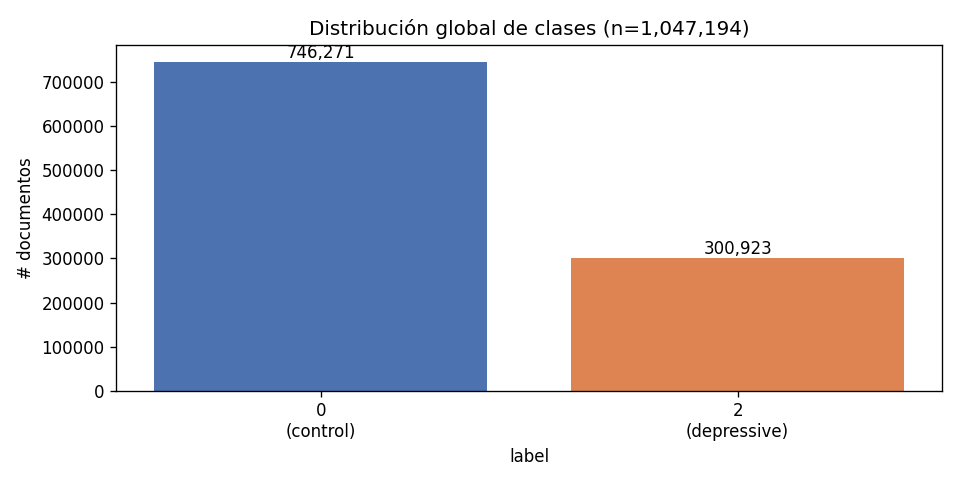
\includegraphics[width=\textwidth]{eda_02_distribucion_clases.png}
        \caption{Documentos por clase.}
    \end{subfigure}
    \hfill
    \begin{subfigure}[t]{0.48\textwidth}
        \centering
        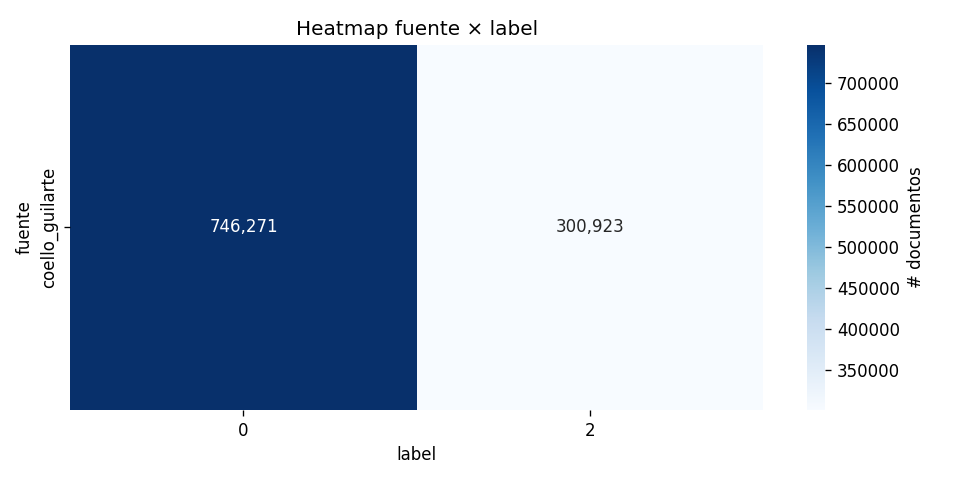
\includegraphics[width=\textwidth]{eda_02_heatmap_fuente_label.png}
        \caption{Fuente por clase.}
    \end{subfigure}
    \caption{Distribución de clases en el corpus nativo Coello-Guilarte.}
    \label{fig:eda_clases}
\end{figure}

\paragraph{Longitud de los textos.} Los tweets son cortos: una media de 59{,}4 caracteres y 11{,}3 tokens (mediana de 10 tokens; percentil 75 de 17; máximo de 61). La distribución por clase (Figura~\ref{fig:eda_longitudes}) muestra que los textos de usuarios depresivos se desplazan hacia longitudes mayores. En una muestra tokenizada con spaCy (\texttt{es\_core\_news\_md}, 50 documentos por clase) la media fue de 9{,}0 tokens en controles y de 20{,}3 en depresivos (Figura~\ref{fig:tokens_spacy}). Los textos traducidos de Reddit son sensiblemente más largos que los tweets, lo que introduce una diferencia de formato entre fuentes.

\begin{figure}[H]
    \centering
    \begin{subfigure}[t]{0.48\textwidth}
        \centering
        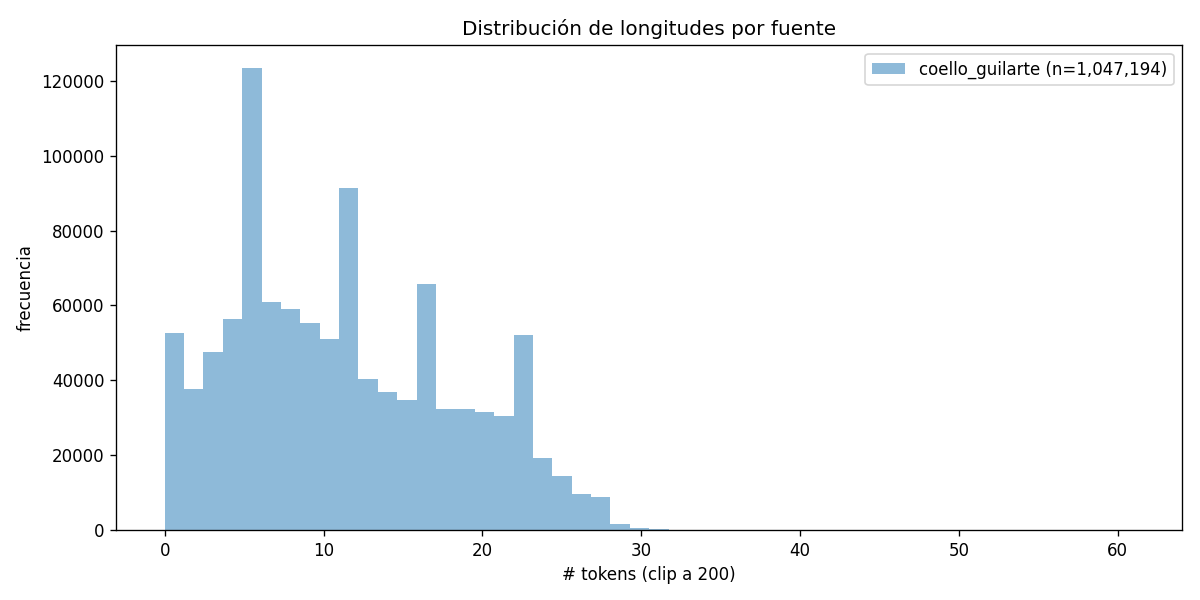
\includegraphics[width=\textwidth]{eda_01_longitudes_por_fuente.png}
        \caption{Longitud en el corpus nativo.}
    \end{subfigure}
    \hfill
    \begin{subfigure}[t]{0.48\textwidth}
        \centering
        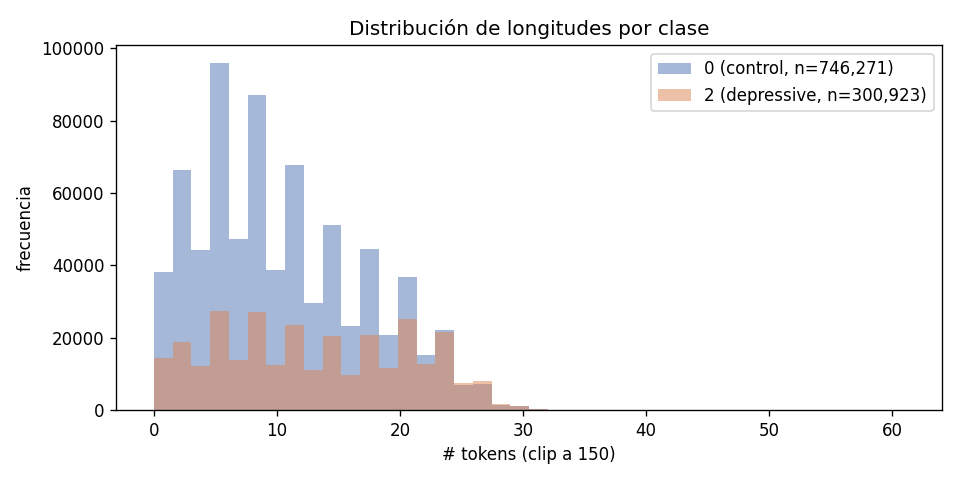
\includegraphics[width=\textwidth]{eda_02_longitudes_por_clase.png}
        \caption{Longitud por clase.}
    \end{subfigure}
    \caption{Longitud de los documentos en tokens.}
    \label{fig:eda_longitudes}
\end{figure}

\begin{figure}[H]
    \centering
    \begin{subfigure}[t]{0.48\textwidth}
        \centering
        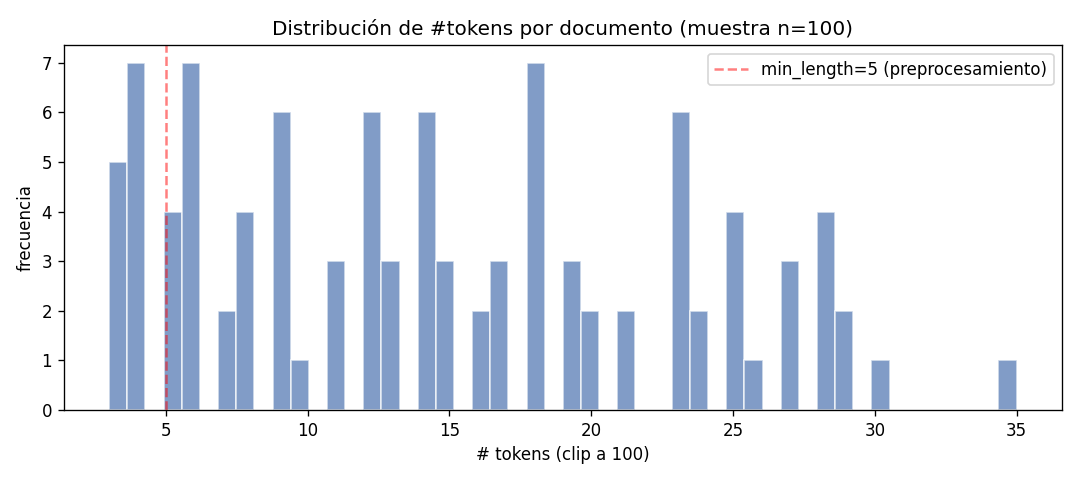
\includegraphics[width=\textwidth]{preprocessing_01_tokens_histogram.png}
        \caption{Histograma de tokens.}
    \end{subfigure}
    \hfill
    \begin{subfigure}[t]{0.48\textwidth}
        \centering
        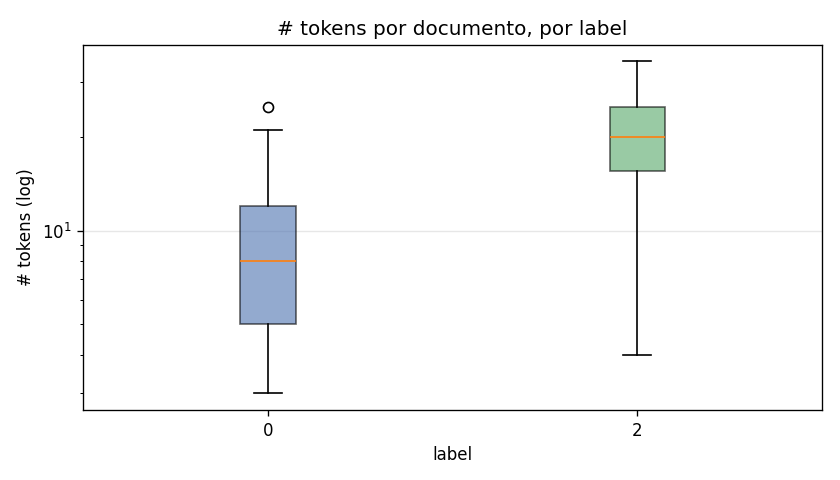
\includegraphics[width=\textwidth]{preprocessing_01_tokens_by_label.png}
        \caption{Tokens por clase (escala logarítmica).}
    \end{subfigure}
    \caption{Tokenización con spaCy sobre una muestra de 100 documentos.}
    \label{fig:tokens_spacy}
\end{figure}

\paragraph{Vocabulario.} Los términos más frecuentes del corpus nativo son palabras funcionales (\emph{de, que, a, la, y, en, el, no}), seguidas de \emph{me} (164\,152 apariciones) y \emph{mi} (84\,184), además del residuo ``\texttt{:}'' mencionado.

\paragraph{Marcadores psicolingüísticos.} Se calcularon frecuencias normalizadas por longitud de cuatro categorías tipo LIWC con lexicones en español (Tabla~\ref{tab:marcadores} y Figura~\ref{fig:marcadores}). Las emociones negativas son un 62\,\% más frecuentes en la clase depresiva y las positivas un 32\,\% menos frecuentes, en línea con la literatura. En cambio, el lenguaje absolutista solo aumenta un 2\,\% y la primera persona del singular es incluso algo \emph{menor} en la clase depresiva. Este último resultado contrasta con los hallazgos clásicos y es coherente con la naturaleza de los datos: la etiqueta se asigna por usuario y la mayoría de sus tweets no hablan de su estado de ánimo.

\begin{table}[H]
\centering
\small
\caption{Marcadores psicolingüísticos normalizados por clase (corpus nativo).}
\label{tab:marcadores}
\begin{tabular}{lrrr}
\toprule
\textbf{Categoría} & \textbf{Control (0)} & \textbf{Depresivo (2)} & \textbf{Variación} \\
\midrule
Primera persona singular & 0{,}01663 & 0{,}01613 & $-3$\,\% \\
Absolutistas             & 0{,}00915 & 0{,}00935 & $+2$\,\% \\
Emoción negativa         & 0{,}00433 & 0{,}00702 & $+62$\,\% \\
Emoción positiva         & 0{,}01272 & 0{,}00860 & $-32$\,\% \\
\midrule
Polaridad media (VADER)  & $-0{,}029$ & $-0{,}052$ & -- \\
\bottomrule
\end{tabular}
\end{table}

\begin{figure}[H]
    \centering
    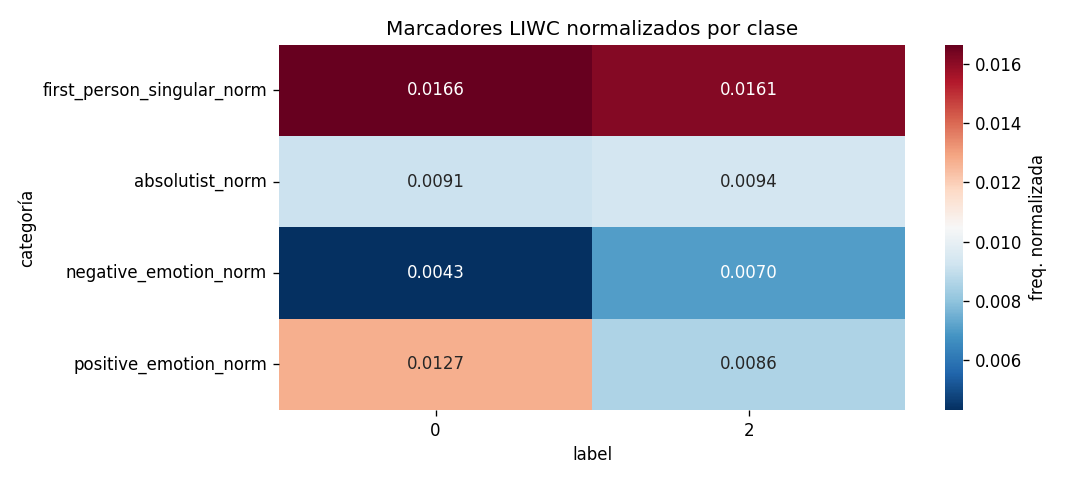
\includegraphics[width=0.75\textwidth]{eda_03_marcadores_por_clase.png}
    \caption{Marcadores psicolingüísticos normalizados por clase.}
    \label{fig:marcadores}
\end{figure}

\paragraph{Polaridad.} La polaridad media calculada con VADER~\cite{hutto2014vader} (con un lexicón en español como respaldo) es más negativa en la clase depresiva ($-0{,}052$ frente a $-0{,}029$), pero la mediana es 0 en ambas clases y la desviación estándar (0{,}21--0{,}25) es un orden de magnitud mayor que la diferencia. VADER fue diseñado para inglés y la mayoría de los tweets en español no contiene términos de su lexicón, por lo que esta señal es débil.

\paragraph{Marcadores diatópicos.} Coello-Guilarte no registra el país de los usuarios, pero su procedencia puede inferirse parcialmente del léxico. Se compiló un lexicón de 175 términos regionales y un patrón morfológico en tres categorías (\path{src/features/lexicons/dialect_markers.yaml}): \emph{dialectismos} (voseo rioplatense, segunda persona del plural peninsular y léxico regional de México, Chile, Colombia y España), \emph{topónimos y gentilicios} (incluidos clubes de fútbol locales) y \emph{figuras políticas} nacionales. En el conjunto de prueba nativo, el 7{,}9\,\% de los tweets contiene al menos un marcador, y su distribución entre clases es desigual (Tabla~\ref{tab:marcadores_dialecto}): los dialectismos aparecen en el 6{,}4\,\% de los tweets depresivos frente al 2{,}7\,\% de los controles, y las figuras políticas en el 1{,}2\,\% frente al 0{,}1\,\%. Esta asimetría anticipa el riesgo planteado en la Sección~\ref{sec:intro_problema}: si la clase está asociada a la región de origen, un clasificador puede aprender a reconocer la procedencia del usuario. El efecto de esos marcadores sobre los modelos se cuantifica en la Sección~\ref{sec:control_dialectal}.

\begin{table}[H]
\centering
\small
\caption{Proporción de tweets del test nativo con al menos un marcador diatópico, por categoría y clase.}
\label{tab:marcadores_dialecto}
\begin{tabular}{lrr}
\toprule
\textbf{Categoría} & \textbf{Control (0)} & \textbf{Depresivo (2)} \\
\midrule
Dialectismos            & 2{,}7\,\% & 6{,}4\,\% \\
Topónimos y gentilicios & 3{,}5\,\% & 4{,}9\,\% \\
Figuras políticas       & 0{,}1\,\% & 1{,}2\,\% \\
\midrule
Usuarios                & 45 & 19 \\
\bottomrule
\end{tabular}
\end{table}

\subsection{Partición a nivel de usuario}
Cuando los textos de un mismo autor se distribuyen entre entrenamiento y prueba, el modelo puede aprender rasgos idiosincráticos de ese autor (temas, muletillas, firmas) y el rendimiento estimado resulta optimista. Para evitarlo, la partición se realizó a nivel de usuario:
\begin{enumerate}[leftmargin=2em]
    \item se calculó la etiqueta modal de cada usuario;
    \item \emph{dentro de cada fuente}, se asignaron usuarios completos a entrenamiento, validación y prueba en proporciones 70/10/20, estratificando por esa etiqueta y con semilla 42;
    \item cada documento heredó la partición de su autor.
\end{enumerate}
Particionar por separado cada fuente garantiza que todas ellas estén representadas en las tres particiones con ambas clases y que la asignación de los usuarios de una fuente no dependa de las demás. En particular, los usuarios de Coello-Guilarte reciben exactamente la misma asignación en el esquema mono-corpus (\texttt{splits}) que en el multi-corpus (\texttt{splits\_multi}), de modo que la porción nativa del conjunto de prueba multi \emph{es} el conjunto de prueba mono. Esto permite comparar todos los modelos sobre un mismo conjunto de prueba nativo. Kaggle SDD no incluye identificadores de autor, por lo que cada publicación se trató como un usuario sintético independiente, el mismo criterio que ya se aplicaba a Depression Reddit. Cada esquema se acompaña de un manifiesto JSON con conteos por partición, clase y fuente (Anexo~\ref{anx:manifiestos}). La Figura~\ref{fig:particion} ilustra el esquema.

\begin{figure}[H]
\centering
\resizebox{0.97\textwidth}{!}{% Partición independiente por fuente: cada corpus se divide 70/10/20 por usuario.
\begin{tikzpicture}[font=\footnotesize, x=1cm, y=1cm]
    % Leyenda
    \node[anchor=west] at (0, 1.3) {%
        \tikz\fill[ugrAzul] (0,0) rectangle (0.3,0.3); Entrenamiento (70\,\%)\qquad
        \tikz\fill[ugrCeleste] (0,0) rectangle (0.3,0.3); Validación (10\,\%)\qquad
        \tikz\fill[ugrNaranja] (0,0) rectangle (0.3,0.3); Prueba (20\,\%)};

    % Barras por fuente
    \foreach \y/\nombre/\info in {
        0/Coello-Guilarte/317 usuarios,
        -1.05/Kaggle SDD/232\,067 usuarios sintéticos,
        -2.1/Reddit MH Posts/20\,242 usuarios,
        -3.15/Depression Reddit/7\,731 usuarios sintéticos} {
        \node[anchor=east, align=right] at (-0.25, \y) {\textbf{\nombre}\\[-1pt] {\color{ugrGris}\info}};
        \fill[ugrAzul]    (0, \y - 0.32) rectangle (7, \y + 0.32);
        \fill[ugrCeleste] (7, \y - 0.32) rectangle (8, \y + 0.32);
        \fill[ugrNaranja] (8, \y - 0.32) rectangle (10, \y + 0.32);
        \draw[white, line width=1.4pt] (7, \y - 0.32) -- (7, \y + 0.32) (8, \y - 0.32) -- (8, \y + 0.32);
        \node[text=white, font=\scriptsize\bfseries] at (3.5, \y) {usuarios completos, estratificados por clase};
    }

    % Test nativo común
    \draw[ugrRojo, line width=1.1pt, dashed, rounded corners=2pt] (7.92, -0.42) rectangle (10.08, 0.42);
    \node[ugrRojo, anchor=south, font=\scriptsize\bfseries] at (9.0, 0.44) {test nativo común};

    % Llaves
    \draw[decorate, decoration={brace, amplitude=5pt}, line width=0.8pt, ugrAzul] (10.35, 0.36) -- (10.35, -0.36)
        node[midway, right=7pt, text=ugrAzul] {\textbf{splits mono}};
    \draw[decorate, decoration={brace, amplitude=7pt}, line width=0.8pt, ugrNaranja!90!black] (12.75, 0.42) -- (12.75, -3.5)
        node[midway, right=9pt, align=left, text=ugrNaranja!90!black] {\textbf{splits multi}\\ unión de las\\ cuatro fuentes};
\end{tikzpicture}
}
\caption{Partición independiente por fuente. Cada corpus se divide por usuarios completos en 70/10/20; \texttt{splits mono} es la fila de Coello-Guilarte y \texttt{splits multi} la unión de las cuatro filas, por lo que la prueba nativa es común a ambos esquemas.}
\label{fig:particion}
\end{figure}

\subsection{Verificación de las particiones}
\label{sec:verificacion}
Antes de interpretar los resultados se auditaron ambos esquemas. La auditoría de una primera versión de \texttt{splits\_multi} detectó un error de diseño que se describe a continuación, porque ilustra un riesgo general de los corpus multifuente.

\paragraph{Error detectado en la primera versión.} En la proyección inicial de Kaggle SDD se había asignado un único identificador de usuario sintético por clase. La partición por usuario envió entonces \emph{todos} los controles de Kaggle (116\,031) a entrenamiento y \emph{todos} sus casos positivos (116\,036) a prueba. Además, como la asignación aleatoria se calculaba sobre el conjunto de todos los usuarios, los usuarios nativos del test multi no coincidían con los del test mono (47 de los 68 habían estado en el entrenamiento mono). El resultado fue un conjunto de prueba con un 55\,\% de casos positivos, un tercio de los cuales pertenecía a un dominio sin ejemplos positivos en entrenamiento, y una comparación entre escenarios hecha sobre conjuntos de prueba distintos. Con esa versión, la Regresión Logística multi parecía mejorar el F1-macro de 0{,}655 a 0{,}713 y el F1 de la clase depresiva de 0{,}546 a 0{,}748; un experimento de control mostró que esa mejora se debía a la composición del conjunto de prueba. Se corrigió la proyección (un usuario por publicación) y la partición (estratificada por fuente), se regeneraron las particiones y se reentrenaron todos los modelos multi. Los resultados de la primera versión se descartaron y se conservan solo como respaldo en el repositorio.

\paragraph{Verificación de la versión final.} La Tabla~\ref{tab:splits} resume ambos esquemas.

\begin{table}[H]
\centering
\small
\caption{Verificación de las particiones finales.}
\label{tab:splits}
\begin{tabular}{llrrrr}
\toprule
\textbf{Esquema} & \textbf{Partición} & \textbf{Filas} & \textbf{Usuarios} & \textbf{\% clase 2} & \textbf{Vacíos} \\
\midrule
\multirow{3}{*}{Mono}  & Entrenamiento & 700\,717 & 221 & 30{,}3 & 1{,}28\,\% \\
                       & Validación    &  95\,630 &  32 & 19{,}0 & 2{,}66\,\% \\
                       & Prueba        & 250\,847 &  64 & 28{,}1 & 1{,}60\,\% \\
\midrule
\multirow{3}{*}{Multi} & Entrenamiento & 885\,381 & 182\,245 & 35{,}3 & 1{,}02\,\% \\
                       & Validación    & 122\,038 &  26\,038 & 26{,}7 & 2{,}09\,\% \\
                       & Prueba        & 303\,604 &  52\,074 & 32{,}7 & 1{,}32\,\% \\
\bottomrule
\end{tabular}
\end{table}

\begin{itemize}[leftmargin=2em]
    \item \textbf{Sin fuga de usuarios.} En ambos esquemas la intersección de usuarios entre entrenamiento, validación y prueba es vacía, y ningún usuario tiene más de una etiqueta. Los conteos coinciden con los manifiestos.
    \item \textbf{Representación por fuente.} Todas las fuentes aparecen en las tres particiones en proporción 70/10/20 y, cuando tienen dos clases, con ambas (Anexo~\ref{anx:manifiestos}).
    \item \textbf{Test nativo común.} La porción Coello-Guilarte del test multi contiene los mismos 64 usuarios y 250\,847 textos que el test mono, y ninguno de ellos pertenece al entrenamiento de ningún esquema. Como control, la Regresión Logística entrenada solo con la porción nativa del entrenamiento multi reproduce exactamente el resultado de la línea base mono (F1-macro 0{,}6528; AUC 0{,}7527).
    \item \textbf{Prevalencia comparable.} La proporción de la clase depresiva en prueba es del 28{,}1\,\% en mono y del 32{,}7\,\% en multi.
    \item \textbf{Textos repetidos.} El 4{,}4\,\% (mono) y el 3{,}7\,\% (multi) de las filas de prueba tienen un texto idéntico a alguno de entrenamiento. Se trata de cadenas triviales de distintos usuarios (``\texttt{:}'', ``\dots'', emojis, ``JAJAJA'') con una longitud media de 33 caracteres, no de duplicados de autor, por lo que no constituyen fuga de información relevante.
    \item \textbf{Pocos usuarios nativos en evaluación.} El conjunto de prueba nativo contiene 64 usuarios. Como la etiqueta es por usuario, la unidad efectiva de muestreo es el usuario y las métricas por documento tienen una incertidumbre mayor de la que sugiere el número de filas.
\end{itemize}

\newpage
% =====================================================================
% 4. METODOLOGÍA
% =====================================================================
\section{Metodología}
\label{sec:metodologia}

\subsection{Diseño general}
La investigación se organizó en seis etapas: (1) revisión bibliográfica; (2) construcción del corpus; (3) preprocesamiento y análisis exploratorio; (4) modelado; (5) evaluación; y (6) interpretabilidad. La Figura~\ref{fig:pipeline} resume el flujo de datos.

\begin{figure}[H]
\centering
\resizebox{\textwidth}{!}{% Pipeline de datos: fuentes -> anonimización -> traducción -> unificación -> partición -> modelado -> evaluación
\begin{tikzpicture}[font=\footnotesize]
    % Fuentes
    \node[nodoES] (c) at (-5.85, 0) {\textbf{Coello-Guilarte}\\ Twitter \textperiodcentered{} español\\ 1\,047\,194 textos};
    \node[nodoEN] (k) at (-1.95, 0) {\textbf{Kaggle SDD}\\ Reddit \textperiodcentered{} inglés\\ 232\,067 textos};
    \node[nodoEN] (m) at ( 1.95, 0) {\textbf{Reddit MH Posts}\\ Reddit \textperiodcentered{} inglés\\ 24\,031 textos};
    \node[nodoEN] (d) at ( 5.85, 0) {\textbf{Depression Reddit}\\ Reddit \textperiodcentered{} inglés\\ 7\,731 textos};

    % Procesamiento
    \node[proceso=15.3cm] (an) at (0, -1.95)
        {\textbf{Limpieza y anonimización}: URLs, menciones, correos y teléfonos; identificadores \emph{hash} SHA-256\\
         \codigo{make\_dataset.py \textperiodcentered{} project\_user\_csvs.py}};
    \node[proceso=11.1cm, draw=ugrNaranja, fill=ugrNaranja!7] (tr) at (1.95, -3.7)
        {\textbf{Traducción EN$\to$ES} con MarianMT (\texttt{opus-mt-en-es}): 263\,829 textos, caché JSONL y control de calidad\\
         \codigo{translation/translate.py}};
    \node[proceso=15.3cm] (un) at (0, -5.45)
        {\textbf{Unificación} en \texttt{corpus\_v1.parquet}: 1\,311\,023 textos de 260\,357 usuarios\\
         \codigo{merge\_corpora.py}};
    \node[proceso=15.3cm] (sp) at (0, -7.2)
        {\textbf{Partición por fuente y por usuario} (70/10/20, estratificada por clase, semilla 42)\\
         \codigo{build\_splits.py}};
    \node[nodoES, text width=7.1cm] (mono) at (-3.95, -8.95)
        {\textbf{splits mono}: solo Coello-Guilarte\\ 700\,717 / 95\,630 / 250\,847 textos};
    \node[nodoEN, text width=7.1cm] (multi) at (3.95, -8.95)
        {\textbf{splits multi}: las cuatro fuentes\\ 885\,381 / 122\,038 / 303\,604 textos};

    % Modelado
    \node[font=\footnotesize\bfseries, text=ugrAzul] (mt) at (0, -10.3) {Modelado (mismos hiperparámetros en ambos esquemas)};
    \node[proceso=4.6cm] (m1) at (-5.2, -11.25) {\textbf{TF-IDF + LR / SVM}\\ submuestreo o ponderación};
    \node[proceso=4.6cm] (m2) at ( 0.0, -11.25) {\textbf{TF-IDF + rasgos}\\ LIWC, polaridad, temporales};
    \node[proceso=4.6cm] (m3) at ( 5.2, -11.25) {\textbf{BETO}\\ ajuste fino, 3 épocas};
    \begin{scope}[on background layer]
        \node[draw=ugrAzul!45, dashed, rounded corners=4pt, fill=ugrAzul!3, inner sep=6pt, fit=(mt)(m1)(m2)(m3)] (grp) {};
    \end{scope}

    % Evaluación
    \node[resultado=7.1cm] (ev) at (-3.95, -13.2)
        {\textbf{Evaluación por fuente}\\ test nativo común y test traducido\\ F1-macro, F1 depresivo, AUC, $\kappa$};
    \node[resultado=7.1cm] (xi) at (3.95, -13.2)
        {\textbf{Interpretabilidad y auditoría}\\ coeficientes del modelo lineal\\ verificación de particiones};

    % Flechas
    \foreach \n in {c, k, m, d} { \draw[flecha] (\n) -- (\n |- an.north); }
    \draw[flecha] (an.south -| c) -- (un.north -| c);
    \foreach \n in {k, m, d} { \draw[flecha] (an.south -| \n) -- (tr.north -| \n); }
    \draw[flecha] (tr) -- (tr |- un.north);
    \draw[flecha] (un) -- (sp);
    \draw[flecha] (sp.south -| mono) -- (mono);
    \draw[flecha] (sp.south -| multi) -- (multi);
    \draw[flecha] (mono) -- (mono |- grp.north);
    \draw[flecha] (multi) -- (multi |- grp.north);
    \draw[flecha] (grp.south -| ev) -- (ev);
    \draw[flecha] (grp.south -| xi) -- (xi);
\end{tikzpicture}
}
\caption{Pipeline de procesamiento. En azul, datos nativos en español; en naranja, datos traducidos; en verde, salidas de evaluación. Bajo cada etapa se indica el módulo del repositorio que la implementa; las cifras de las particiones corresponden a entrenamiento, validación y prueba.}
\label{fig:pipeline}
\end{figure}

\subsection{Preprocesamiento y extracción de características}
\paragraph{Texto.} Los modelos trabajan sobre la columna \texttt{text\_clean} (texto anonimizado). No se aplicó lematización ni eliminación de \emph{stopwords} para los modelos finales: los pronombres y las palabras funcionales forman parte de los marcadores de interés y BETO requiere el texto original.

\paragraph{Rasgos psicolingüísticos.} Para el modelo combinado se calcularon 19 rasgos por documento:
\begin{itemize}[leftmargin=2em]
    \item conteos normalizados de primera persona del singular, absolutistas, emoción negativa y emoción positiva, a partir de lexicones en español (\texttt{src/features/lexicons/});
    \item polaridad con VADER y lexicón de respaldo en español;
    \item rasgos temporales derivados de la marca de tiempo (hora del día, día de la semana, publicación nocturna e intervalo entre mensajes).
\end{itemize}
Se excluyó deliberadamente el número de mensajes por usuario, porque calculado dentro de cada partición mide el tamaño de la partición y no la actividad real del usuario, lo que habría introducido una fuga.

\subsection{Estrategias de balanceo de clases}
Para que los clasificadores no colapsen hacia la clase mayoritaria se evaluaron dos estrategias, aplicadas solo al conjunto de entrenamiento:
\begin{enumerate}[leftmargin=2em]
    \item \textbf{Submuestreo de la clase mayoritaria (50/50).} Se toma una muestra aleatoria de controles del mismo tamaño que la clase positiva: 424\,436 filas en mono (212\,218 por clase) y 625\,862 en multi (312\,931 por clase).
    \item \textbf{Ponderación de clases.} Se entrena con todo el conjunto (700\,717 filas en mono y 885\,381 en multi) ponderando la pérdida de forma inversamente proporcional a la frecuencia de cada clase (\texttt{class\_weight="balanced"}).
\end{enumerate}
Validación y prueba conservan siempre su distribución original.

\subsection{Líneas base clásicas}
\paragraph{TF-IDF.} Unigramas y bigramas, un máximo de 15\,000 términos, frecuencia mínima de documento de 2 y escalado sublineal de la frecuencia.

\paragraph{Regresión Logística.} Implementada con scikit-learn~\cite{pedregosa2011scikit}. Optimizador L-BFGS, regularización $L_2$ con $C=1{,}0$ y hasta 1\,000 iteraciones.

\paragraph{SVM lineal.} \texttt{LinearSVC} con $C=1{,}0$, ponderación de clases y hasta 2\,000 iteraciones, entrenada sobre el conjunto mono completo.

\paragraph{Modelo combinado.} TF-IDF y los 19 rasgos psicolingüísticos (estandarizados) se concatenan mediante un \texttt{ColumnTransformer} y alimentan una Regresión Logística con los mismos hiperparámetros, entrenada sobre el conjunto mono submuestreado para compararla en igualdad de condiciones con la línea base.

\subsection{Ajuste fino de BETO}
Se ajustó \texttt{dccuchile/bert-base-spanish-wwm-cased} con una capa lineal de clasificación sobre el token \texttt{[CLS]}, utilizando la biblioteca \texttt{transformers}~\cite{wolf2020transformers}. La configuración, idéntica para mono y multi, se resume en la Tabla~\ref{tab:hiper_beto}. El entrenamiento se realizó sobre el conjunto submuestreado 50/50 para evitar ponderar la pérdida. La Figura~\ref{fig:beto} resume la arquitectura.

\begin{figure}[H]
\centering
\resizebox{\textwidth}{!}{% Arquitectura del ajuste fino de BETO para clasificación binaria.
\begin{tikzpicture}[font=\footnotesize, node distance=0.55cm]
    \node[proceso=2.6cm, fill=ugrGris!8, draw=ugrGris] (tx) {\textbf{Texto}\\ \emph{``no me}\\ \emph{siento bien''}};
    \node[proceso=2.6cm, right=of tx] (tok) {\textbf{Tokenización}\\ WordPiece\\ \texttt{[CLS]} \dots{} \texttt{[SEP]}\\ máx.\ 128 tokens};
    \node[proceso=2.9cm, right=of tok, minimum height=2.6cm, fill=ugrAzul!10, line width=0.9pt] (enc)
        {\textbf{BETO}\\ codificador Transformer\\ 12 capas \texttimes{} 12 cabezas\\ $d = 768$\\ {\color{ugrGris}\scriptsize preentrenado, se ajusta}};
    \node[proceso=2.2cm, right=of enc] (cls) {\textbf{Vector}\\ $h_{\texttt{[CLS]}} \in \mathbb{R}^{768}$};
    \node[proceso=2.2cm, right=of cls, draw=ugrNaranja, fill=ugrNaranja!8] (lin) {\textbf{Capa lineal}\\ $768 \to 2$\\ + softmax};
    \node[resultado=2.9cm, below=0.7cm of lin] (out) {$P(\text{depresivo}\mid x)$};

    \draw[flecha] (tx) -- (tok);
    \draw[flecha] (tok) -- (enc);
    \draw[flecha] (enc) -- (cls);
    \draw[flecha] (cls) -- (lin);
    \draw[flecha] (lin) -- (out);
    \node[below=0.15cm of enc, font=\scriptsize, text=ugrGris, align=center] {AdamW, $\eta = 2\times10^{-5}$, lote 16, FP16};
\end{tikzpicture}
}
\caption{Arquitectura del ajuste fino de BETO. Todos los pesos del codificador se actualizan durante el entrenamiento junto con la capa lineal de clasificación.}
\label{fig:beto}
\end{figure}

\begin{table}[H]
\centering
\small
\caption{Hiperparámetros del ajuste fino de BETO.}
\label{tab:hiper_beto}
\begin{tabular}{ll}
\toprule
\textbf{Parámetro} & \textbf{Valor} \\
\midrule
Longitud máxima de secuencia & 128 tokens \\
Tamaño de lote (entrenamiento / evaluación) & 16 / 32 \\
Optimizador & AdamW \\
Tasa de aprendizaje & $2\times10^{-5}$ con calentamiento lineal (10\,\%) \\
Decaimiento de pesos & 0{,}01 \\
Épocas & 3, evaluación por época \\
Selección de modelo & mejor F1-macro en validación \\
Parada temprana & paciencia de 2 épocas \\
Precisión & mixta (FP16) \\
Semilla & 42 \\
Hardware & NVIDIA RTX 3060 Ti (8\,GB) \\
\bottomrule
\end{tabular}
\end{table}

\subsection{Protocolo de evaluación y métricas}
Todos los modelos se evaluaron sobre los conjuntos de validación y prueba de su esquema, nunca utilizados durante el entrenamiento. Dada la asimetría de clases, se reporta una batería de métricas:
\begin{align}
\text{Precisión} &= \frac{TP}{TP + FP}, \qquad \text{Exhaustividad} = \frac{TP}{TP + FN}, \\
\text{F1} &= 2 \cdot \frac{\text{Precisión} \cdot \text{Exhaustividad}}{\text{Precisión} + \text{Exhaustividad}}, \\
\text{F1-macro} &= \tfrac{1}{2}\left(\text{F1}_{\text{control}} + \text{F1}_{\text{depresión}}\right), \\
\kappa &= \frac{p_o - p_e}{1 - p_e},
\end{align}
donde $p_o$ es la concordancia observada y $p_e$ la esperada por azar~\cite{cohen1960kappa}. Se reporta además la exactitud, el F1 ponderado y el área bajo la curva ROC (AUC) con la clase depresiva como positiva. El F1-macro es la métrica principal porque pondera por igual ambas clases; el AUC es la métrica más robusta a cambios de prevalencia porque no depende del umbral de decisión. Para la SVM lineal, que no estima probabilidades, el AUC se calcula sobre el valor de su función de decisión, ya que la métrica solo requiere un orden de los documentos.

\subsection{Incertidumbre estadística}
\label{sec:incertidumbre}
Como la etiqueta es del usuario y no del documento, las publicaciones de un mismo autor no son observaciones independientes: el conjunto de prueba nativo tiene 250\,847 tweets pero solo 64 usuarios, y uno de ellos aporta por sí solo el 20\,\% de las filas. Por eso la incertidumbre se estimó mediante \emph{bootstrap} por conglomerados: en cada una de 2\,000 réplicas se remuestrean usuarios con reemplazo, estratificando por su etiqueta, y se recalculan todas las métricas sobre los documentos de los usuarios seleccionados. Se reportan intervalos de confianza percentiles del 95\,\%. Para comparar dos modelos se utilizan las mismas réplicas para ambos y se reporta el intervalo de la diferencia, junto con la proporción de réplicas en que el primero supera al segundo. Se considera que una diferencia es estadísticamente distinguible de cero cuando su intervalo no contiene el cero. El procedimiento se implementó en \texttt{src/evaluation/bootstrap.py} y se aplica sin reentrenar ningún modelo, sobre las predicciones guardadas.

\subsection{Evaluación a nivel de usuario}
\label{sec:met_usuario}
Para acercar la evaluación a la unidad de interés clínico, las predicciones por documento se agregan por usuario de dos maneras: el score medio del usuario (con el mismo umbral del modelo) y la proporción de sus textos clasificados como depresivos (voto mayoritario). Las métricas se calculan entonces sobre 64 usuarios, con intervalos obtenidos por \emph{bootstrap} de usuarios. Esta agregación solo es informativa en Coello-Guilarte, donde cada usuario tiene en promedio unos 3\,900 tweets en prueba; en las fuentes de Reddit casi cada publicación tiene su propio usuario.

\subsection{Control experimental del atajo dialectal}
\label{sec:met_dialecto}
Para cuantificar cuánto dependen los modelos de los marcadores diatópicos, cada modelo ya entrenado se volvió a evaluar sobre el test nativo con esos marcadores enmascarados. Cada coincidencia de palabra completa del lexicón se reemplazó por \texttt{[UNK]}, un símbolo neutro para ambos tipos de modelo: TF-IDF lo descarta porque no forma parte de su vocabulario y BETO lo interpreta como su token desconocido. Se evaluaron cuatro condiciones: todas las categorías juntas y cada categoría por separado.

Quitar palabras de un texto puede degradar el rendimiento por la simple pérdida de información. Para separar ese efecto se incluyó un \emph{control aleatorio}: a cada tweet se le enmascara la misma cantidad de palabras que marcadores contenía, pero elegidas al azar entre las que no son marcadores. Si la caída se debe al contenido regional de los marcadores, el enmascarado dirigido debe degradar el rendimiento y el aleatorio no.

Esta prueba mide la dependencia de los modelos \emph{actuales} respecto de esos términos; no equivale a entrenar un modelo sin ellos, que podría compensar con otras señales correlacionadas con la región. El reentrenamiento sobre texto enmascarado queda como trabajo futuro.

\subsection{Interpretabilidad}
Se adoptó la siguiente definición operacional: un modelo es interpretable en la medida en que un observador puede identificar qué características del texto determinan sus predicciones y contrastarlas con conocimiento experto. Se operacionalizó a dos niveles:
\begin{itemize}[leftmargin=2em]
    \item \textbf{Interpretabilidad global de los modelos lineales.} Se analizaron los coeficientes de la Regresión Logística sobre TF-IDF y se contrastaron con los marcadores psicolingüísticos de la literatura. Además de inspeccionar los términos de mayor peso hacia cada clase, se midió si los términos de cada categoría del lexicón aparecen entre los 500 unigramas con mayor coeficiente depresivo más de lo esperable por azar (prueba exacta de Fisher) y si sus coeficientes son mayores que los del resto del vocabulario (prueba de Mann-Whitney). Este es el alcance con que se contrasta \Hs{3}.
    \item \textbf{Auditoría de atajos para todos los modelos.} La prueba de enmascarado de la Sección~\ref{sec:met_dialecto} permite evaluar también a BETO, cuyo funcionamiento interno no se inspeccionó directamente. La interpretabilidad \emph{post hoc} de BETO mediante SHAP o LIME no se implementó por su costo computacional sobre 250\,847 textos y queda como trabajo futuro.
\end{itemize}

\subsection{Replicabilidad}
Se definió la replicabilidad como la posibilidad de que un tercero reproduzca cada paso del pipeline y obtenga los mismos resultados. El código está disponible públicamente en \url{https://github.com/giulicrenna/Deteccion-Temprana-Depresion}. La replicabilidad se operacionalizó mediante:
\begin{enumerate}[leftmargin=2em]
    \item semillas fijas (42) en Python, NumPy, scikit-learn y PyTorch (\texttt{src/utils/seeds.py});
    \item dependencias declaradas en los archivos de requisitos de \texttt{pip} y en el entorno de \texttt{conda} (\path{environment.yml});
    \item hiperparámetros externalizados en archivos YAML (\texttt{configs/});
    \item un \texttt{Makefile} con un objetivo por etapa (Anexo~\ref{anx:reproduccion});
    \item manifiestos JSON con conteos por partición y \emph{hashes} SHA-256 de los archivos descargados;
    \item un registro único de métricas (\texttt{reports/tables/all\_models\_metrics.csv}) con fecha y configuración de cada experimento;
    \item pruebas automáticas con \texttt{pytest} sobre los módulos de modelos y evaluación;
    \item predicciones de prueba unificadas por documento (\texttt{reports/predictions/}) a partir de las cuales un único comando (\texttt{python -m src.evaluation.run\_validation}) recalcula todas las métricas, intervalos y comparaciones del Capítulo~\ref{sec:resultados} sin reentrenar.
\end{enumerate}

\newpage
% =====================================================================
% 5. RESULTADOS Y DISCUSIÓN
% =====================================================================
\section{Resultados y discusión}
\label{sec:resultados}

\subsection{Comparación de modelos sobre el test nativo}
Todos los modelos se evaluaron sobre el mismo conjunto de prueba nativo (250\,847 tweets de 64 usuarios de Coello-Guilarte, 28{,}1\,\% depresivos), que es a la vez el conjunto de prueba mono y la porción nativa del conjunto de prueba multi. La Tabla~\ref{tab:leaderboard} reúne los resultados.

\begin{table}[H]
\centering
\footnotesize
\setlength{\tabcolsep}{4pt}
\caption{Resultados sobre el test nativo común (250\,847 textos). ``Datos'' indica el corpus de entrenamiento.}
\label{tab:leaderboard}
\begin{tabular}{lllrrrrr}
\toprule
\textbf{Datos} & \textbf{Modelo} & \textbf{Balanceo} & \textbf{Acc.} & \textbf{F1-macro} & \textbf{F1 dep.} & \textbf{AUC} & \textbf{$\kappa$} \\
\midrule
\multirow{5}{*}{Mono}
 & LR TF-IDF             & Submuestreo & 0{,}687 & 0{,}653 & 0{,}544 & 0{,}753 & 0{,}317 \\
 & LR TF-IDF             & Ponderación & 0{,}690 & 0{,}655 & 0{,}546 & 0{,}755 & 0{,}321 \\
 & SVM TF-IDF            & Ponderación & 0{,}688 & 0{,}653 & 0{,}544 & 0{,}754 & 0{,}318 \\
 & LR TF-IDF + rasgos    & Submuestreo & 0{,}674 & 0{,}644 & 0{,}540 & 0{,}750 & 0{,}303 \\
 & \cellcolor{filaResaltada}BETO & \cellcolor{filaResaltada}Submuestreo & \cellcolor{filaResaltada}\textbf{0{,}755} & \cellcolor{filaResaltada}\textbf{0{,}717} & \cellcolor{filaResaltada}\textbf{0{,}613} & \cellcolor{filaResaltada}\textbf{0{,}808} & \cellcolor{filaResaltada}\textbf{0{,}437} \\
\midrule
\multirow{2}{*}{Multi}
 & LR TF-IDF             & Submuestreo & 0{,}712 & 0{,}648 & 0{,}499 & 0{,}719 & 0{,}297 \\
 & BETO                  & Submuestreo & 0{,}740 & 0{,}701 & 0{,}594 & 0{,}796 & 0{,}407 \\
\bottomrule
\end{tabular}

\vspace{0.15cm}
{\footnotesize La SVM lineal se optimizó con pérdida \emph{hinge} y no estima probabilidades; su AUC se calculó sobre el valor de la función de decisión. El F1 de la clase depresiva no había sido registrado por el pipeline original de líneas base y se recalculó a partir del modelo guardado, sin reentrenarlo.}
\end{table}

La Tabla~\ref{tab:leaderboard_ic} agrega los intervalos de confianza del 95\,\% obtenidos por \emph{bootstrap} de usuarios (Sección~\ref{sec:incertidumbre}). Con solo 64 usuarios en prueba los intervalos son amplios (unos $\pm 0{,}05$ en F1-macro y en AUC), mucho más de lo que sugeriría el número de textos.

\begin{table}[H]
\centering
\footnotesize
\setlength{\tabcolsep}{4pt}
\caption{Métricas sobre el test nativo con intervalos de confianza del 95\,\% (\emph{bootstrap} de 64 usuarios, 2\,000 réplicas). La LR mono corresponde a la variante con ponderación.}
\label{tab:leaderboard_ic}
\begin{tabular}{llcccc}
\toprule
\textbf{Datos} & \textbf{Modelo} & \textbf{F1-macro} & \textbf{F1 dep.} & \textbf{AUC} & \textbf{$\kappa$} \\
\midrule
\multirow{3}{*}{Mono}
 & LR TF-IDF               & 0{,}655 {\scriptsize [0{,}606; 0{,}693]} & 0{,}546 {\scriptsize [0{,}431; 0{,}638]} & 0{,}755 {\scriptsize [0{,}718; 0{,}790]} & 0{,}321 {\scriptsize [0{,}241; 0{,}390]} \\
 & SVM TF-IDF              & 0{,}653 {\scriptsize [0{,}605; 0{,}692]} & 0{,}544 {\scriptsize [0{,}429; 0{,}638]} & 0{,}754 {\scriptsize [0{,}716; 0{,}787]} & 0{,}318 {\scriptsize [0{,}238; 0{,}388]} \\
 & BETO                    & 0{,}717 {\scriptsize [0{,}665; 0{,}759]} & 0{,}613 {\scriptsize [0{,}498; 0{,}703]} & 0{,}808 {\scriptsize [0{,}755; 0{,}849]} & 0{,}437 {\scriptsize [0{,}339; 0{,}519]} \\
\midrule
\multirow{2}{*}{Multi}
 & LR TF-IDF               & 0{,}648 {\scriptsize [0{,}614; 0{,}674]} & 0{,}499 {\scriptsize [0{,}410; 0{,}573]} & 0{,}719 {\scriptsize [0{,}680; 0{,}752]} & 0{,}297 {\scriptsize [0{,}231; 0{,}349]} \\
 & BETO                    & 0{,}701 {\scriptsize [0{,}650; 0{,}745]} & 0{,}594 {\scriptsize [0{,}478; 0{,}686]} & 0{,}796 {\scriptsize [0{,}746; 0{,}836]} & 0{,}407 {\scriptsize [0{,}312; 0{,}491]} \\
\bottomrule
\end{tabular}
\end{table}

Los intervalos de los modelos se superponen, pero eso no impide distinguirlos: como todos se evalúan sobre los mismos usuarios, la comparación pertinente es la de la diferencia pareada, cuya varianza es mucho menor porque la dificultad de cada usuario afecta a ambos modelos por igual. La Tabla~\ref{tab:diferencias} resume esas diferencias.

\begin{table}[H]
\centering
\footnotesize
\setlength{\tabcolsep}{4pt}
\caption{Diferencias pareadas sobre el test nativo (A $-$ B) con intervalos de confianza del 95\,\% por \emph{bootstrap} de usuarios.}
\label{tab:diferencias}
\begin{tabular}{llccc}
\toprule
\textbf{A} & \textbf{B} & \textbf{$\Delta$ F1-macro} & \textbf{$\Delta$ AUC} & \textbf{$\Delta\,\kappa$} \\
\midrule
BETO mono  & LR mono    & $+0{,}062$ {\scriptsize [0{,}038; 0{,}081]} & $+0{,}052$ {\scriptsize [0{,}024; 0{,}077]} & $+0{,}116$ {\scriptsize [0{,}068; 0{,}155]} \\
BETO mono  & SVM mono   & $+0{,}063$ {\scriptsize [0{,}040; 0{,}081]} & $+0{,}054$ {\scriptsize [0{,}026; 0{,}077]} & $+0{,}119$ {\scriptsize [0{,}072; 0{,}156]} \\
BETO multi & LR multi   & $+0{,}053$ {\scriptsize [0{,}019; 0{,}092]} & $+0{,}077$ {\scriptsize [0{,}047; 0{,}109]} & $+0{,}110$ {\scriptsize [0{,}046; 0{,}184]} \\
\midrule
BETO multi & BETO mono  & $-0{,}016$ {\scriptsize [$-0{,}035$; $-0{,}004$]} & $-0{,}012$ {\scriptsize [$-0{,}019$; $-0{,}004$]} & $-0{,}030$ {\scriptsize [$-0{,}067$; $-0{,}008$]} \\
LR multi   & LR mono\textsuperscript{a} & $-0{,}004$ {\scriptsize [$-0{,}031$; 0{,}022]} & $-0{,}033$ {\scriptsize [$-0{,}049$; $-0{,}022$]} & $-0{,}021$ {\scriptsize [$-0{,}063$; 0{,}018]} \\
\bottomrule
\end{tabular}

\vspace{0.15cm}
{\footnotesize \textsuperscript{a} Regresión Logística con submuestreo entrenada solo con la porción nativa del entrenamiento multi, que reproduce la línea base mono (Sección~\ref{sec:verificacion}).}
\end{table}

\paragraph{Modelos léxicos.} Las dos estrategias de balanceo producen resultados prácticamente idénticos (F1-macro 0{,}653 y 0{,}655), y la SVM lineal no mejora a la Regresión Logística. Con un 40\,\% menos de datos, el submuestreo alcanza el mismo rendimiento que la ponderación, lo que indica que el límite del modelo léxico no es la cantidad de ejemplos. Por esa razón, en el escenario multi solo se entrenó la variante con submuestreo.

\paragraph{Modelo contextual.} BETO mono mejora a la mejor línea base en 6{,}2 puntos de F1-macro, 6{,}7 de F1 depresivo, 5{,}2 de AUC y 0{,}12 de $\kappa$. Las cuatro diferencias tienen intervalos de confianza enteramente positivos y BETO supera a la línea base en el 100\,\% de las réplicas (Tabla~\ref{tab:diferencias}), por lo que la ventaja no se explica por la variabilidad entre usuarios. Su matriz de confusión en prueba (Figura~\ref{fig:cm_beto}) arroja una exhaustividad del 68{,}9\,\% para la clase depresiva, con una precisión del 55{,}2\,\% y una especificidad del 78{,}1\,\%. La ventaja se mantiene entre los modelos multi: BETO multi supera a la Regresión Logística multi en 5{,}3 puntos de F1-macro y 7{,}7 de AUC. La Figura~\ref{fig:roc_nativo} muestra que la curva ROC de ambos BETO domina a la de ambas regresiones en todo el rango de umbrales.

\begin{figure}[H]
    \centering
    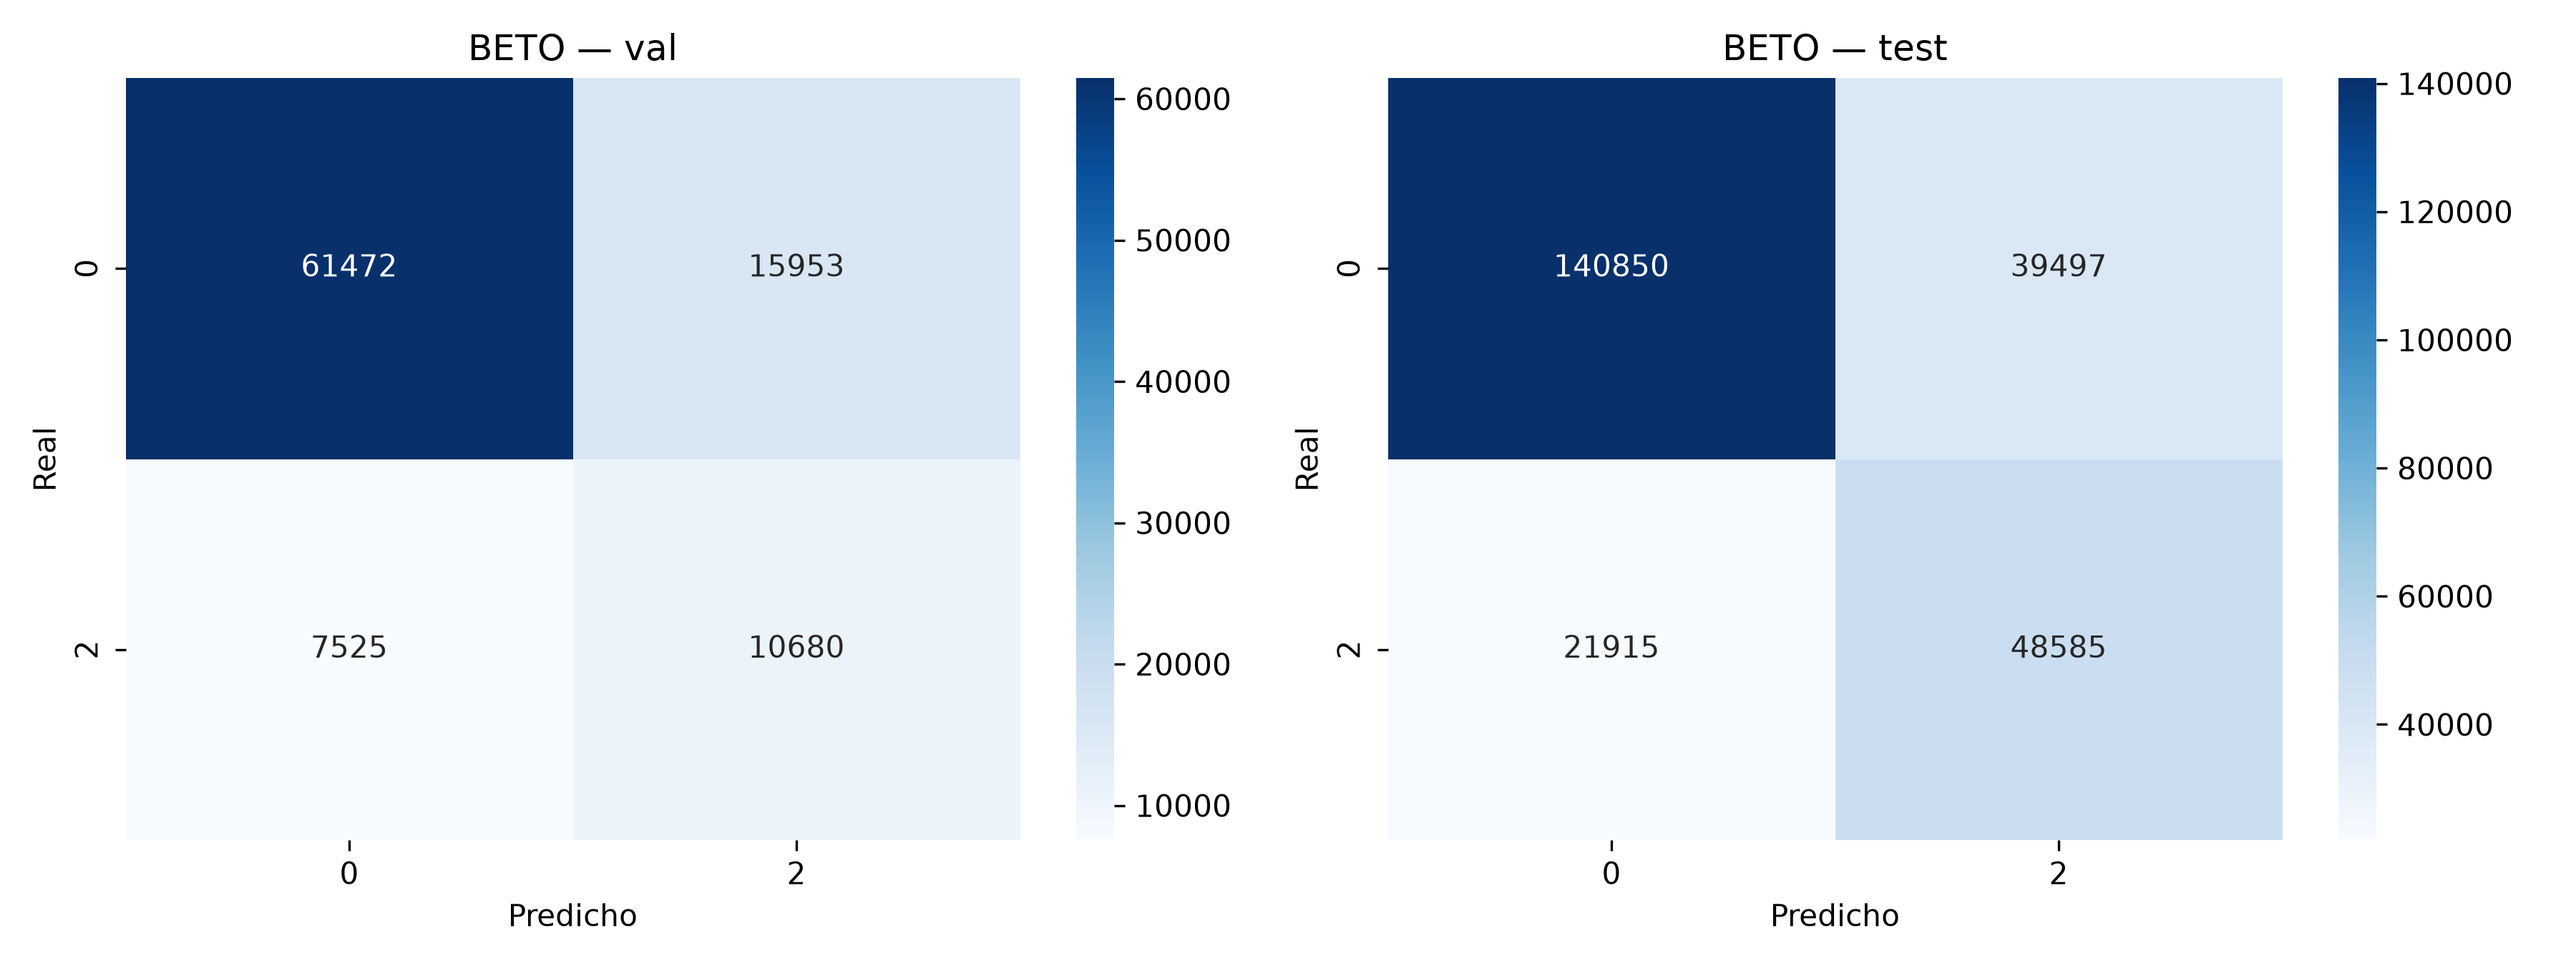
\includegraphics[width=0.9\textwidth]{beto_confusion_matrix.png}
    \caption{Matrices de confusión de BETO mono en validación y prueba (0: control; 2: depresivo).}
    \label{fig:cm_beto}
\end{figure}

\begin{figure}[H]
    \centering
    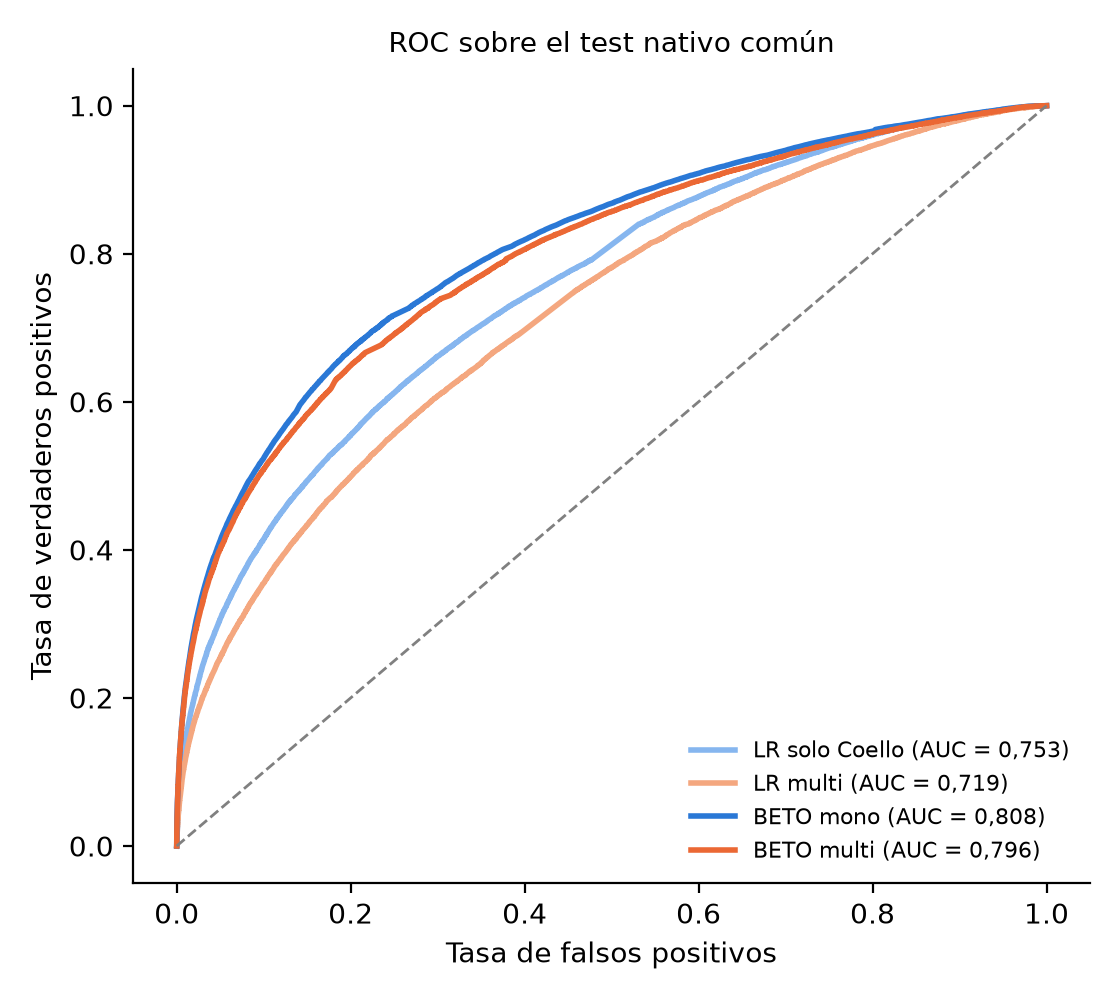
\includegraphics[width=0.62\textwidth]{roc_test_nativo.png}
    \caption{Curvas ROC de los cuatro modelos principales sobre el test nativo común.}
    \label{fig:roc_nativo}
\end{figure}

\paragraph{Brecha entre validación y prueba.} En el escenario mono, BETO obtuvo un F1-macro de 0{,}658 en validación y de 0{,}717 en prueba. La diferencia no indica un error: el conjunto de validación tiene solo 32 usuarios y un 19\,\% de casos positivos, frente a 64 usuarios y un 28\,\% en prueba. Con tan pocos usuarios, la composición de cada partición influye notablemente en las métricas.

\subsection{Dinámica del entrenamiento de BETO}
La Figura~\ref{fig:curvas_beto} muestra la evolución del entrenamiento mono. La pérdida de entrenamiento desciende de forma escalonada al inicio de cada época (de unos 0{,}45 a 0{,}35 y luego a 0{,}27), mientras que la pérdida de validación crece de 0{,}565 a 0{,}585 y a 0{,}778. El F1-macro de validación alcanza su máximo en la segunda época (0{,}658) y desciende en la tercera (0{,}651), un patrón de sobreajuste a partir de la segunda época. La selección del mejor punto de control según el F1-macro de validación retuvo el modelo de la época 2. El entrenamiento demandó 8\,050 segundos (unas 2{,}2 horas) y la inferencia procesó unos 717 textos por segundo.

\begin{figure}[H]
    \centering
    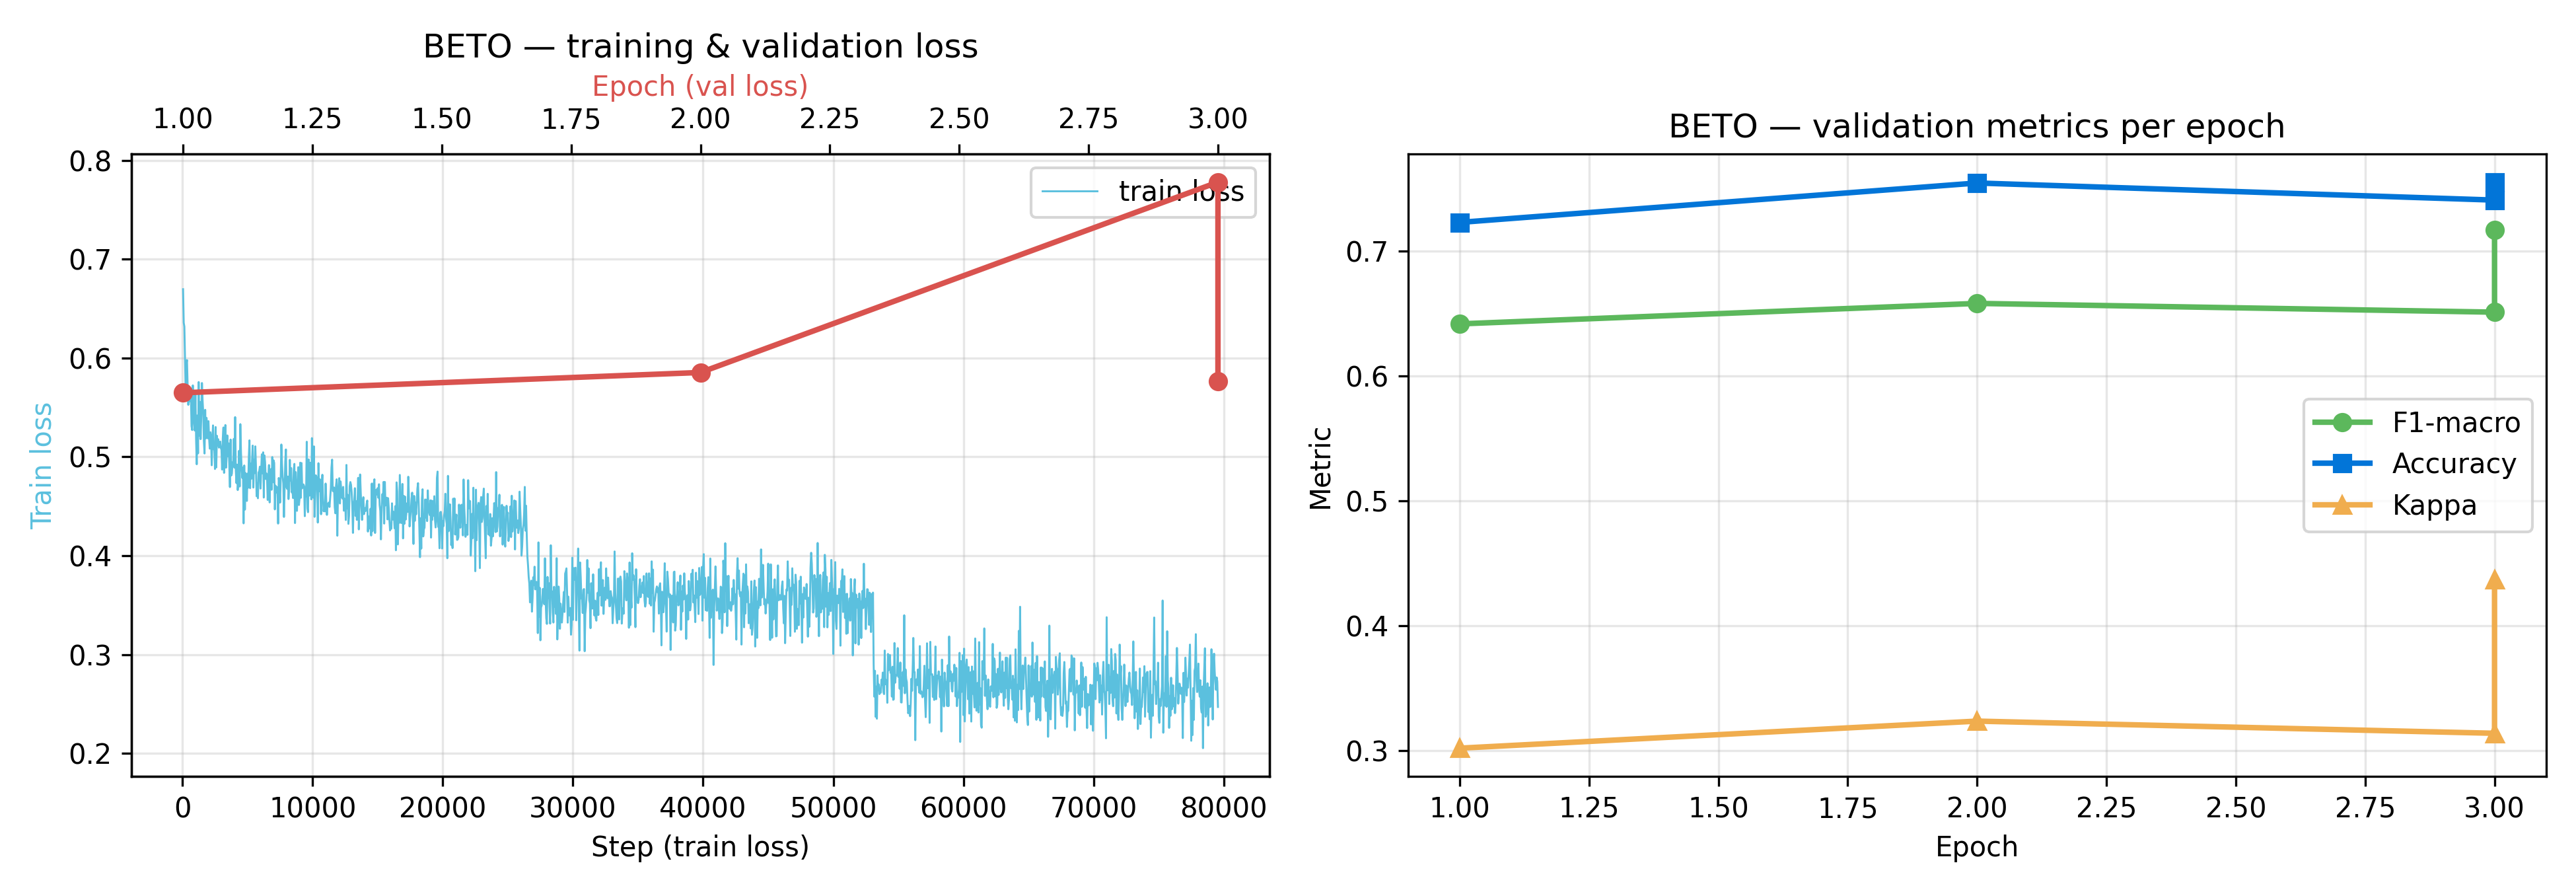
\includegraphics[width=\textwidth]{beto_training_curves.png}
    \caption{Curvas de entrenamiento de BETO mono. Izquierda: pérdida de entrenamiento por paso y de validación por época. Derecha: métricas de validación por época; el último punto de cada serie corresponde a la evaluación en prueba del modelo seleccionado.}
    \label{fig:curvas_beto}
\end{figure}

El entrenamiento multi (625\,862 textos tras el submuestreo, 117\,351 pasos) muestra la misma dinámica (Figura~\ref{fig:curvas_beto_multi}): la pérdida de entrenamiento cae de unos 0{,}37 a 0{,}31 y a 0{,}23, mientras que la de validación sube de 0{,}470 a 0{,}526 y a 0{,}626. En este caso, sin embargo, el F1-macro de validación apenas varía (0{,}739; 0{,}737; 0{,}747) y la selección retuvo la época 3. Que la pérdida de validación crezca mientras el F1 se mantiene indica que el modelo gana confianza en sus predicciones (probabilidades más extremas) sin mejorar su capacidad de separación; el número de épocas podría reducirse a una sin pérdida apreciable de rendimiento.

\begin{figure}[H]
    \centering
    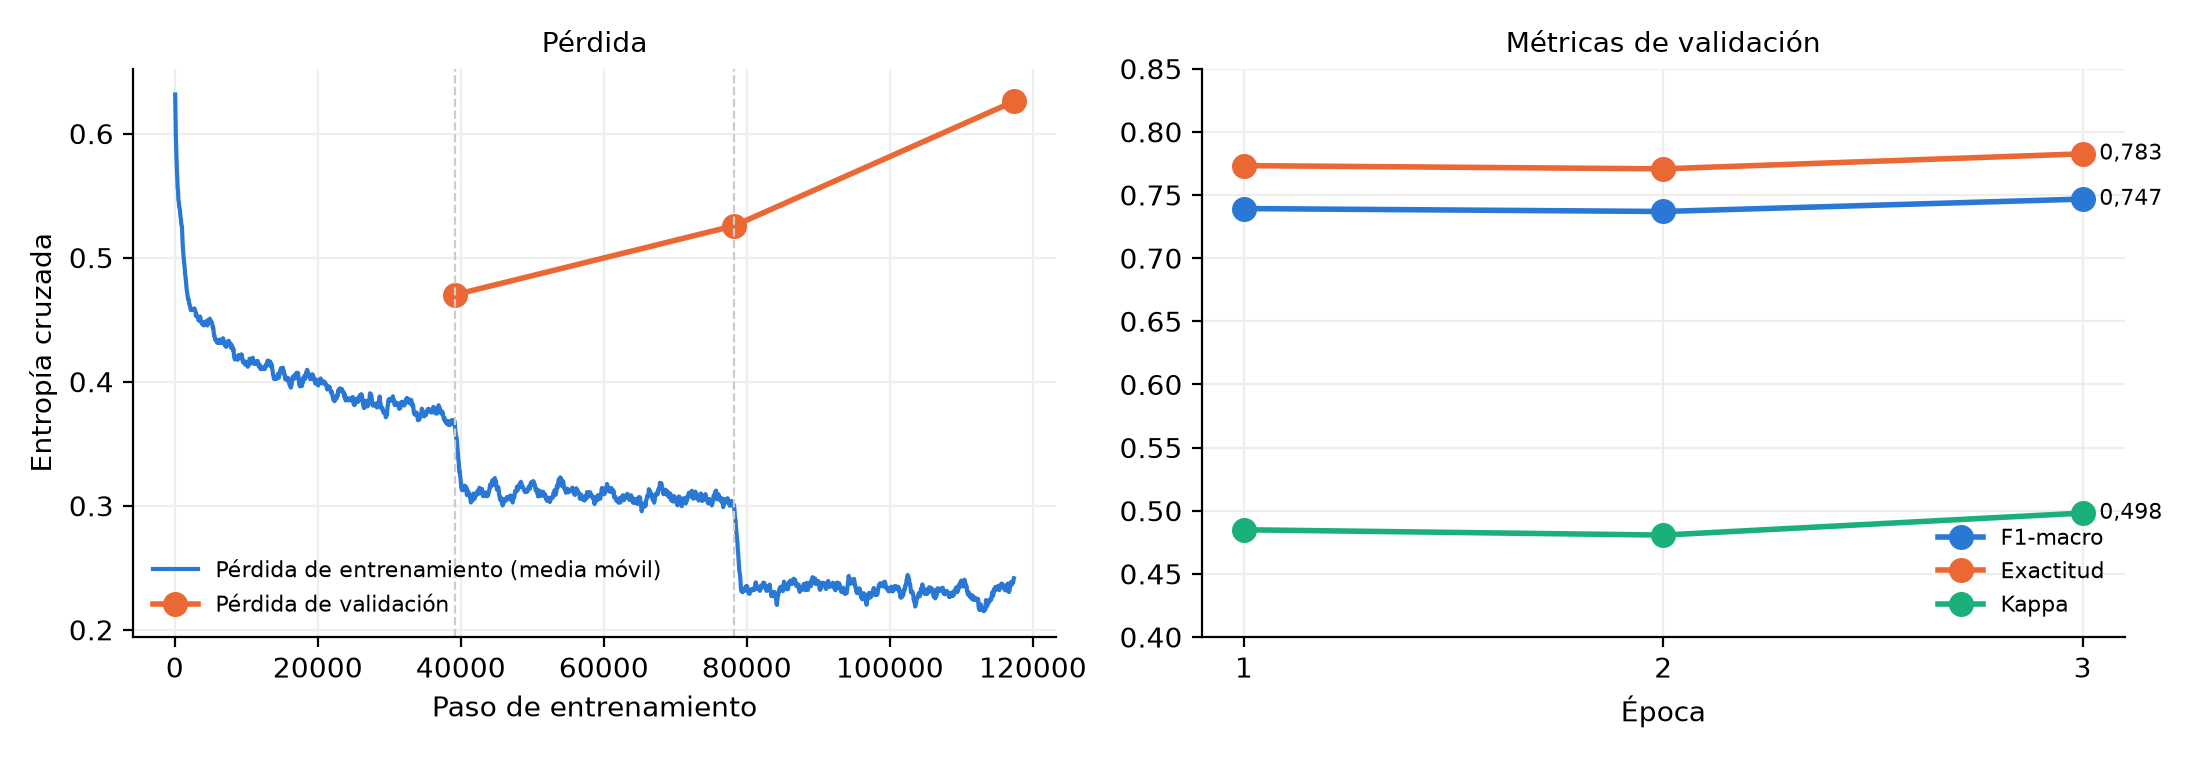
\includegraphics[width=\textwidth]{beto_multi_training_curves.png}
    \caption{Curvas de entrenamiento de BETO multi. Izquierda: pérdida de entrenamiento (media móvil) y de validación; las líneas punteadas marcan el fin de cada época. Derecha: métricas de validación por época.}
    \label{fig:curvas_beto_multi}
\end{figure}

\subsection{Rasgos psicolingüísticos combinados}
Añadir los 19 rasgos psicolingüísticos y temporales a TF-IDF \emph{redujo} el F1-macro de 0{,}653 a 0{,}644 y el AUC de 0{,}753 a 0{,}750. La matriz de confusión (Figura~\ref{fig:cm_combined}) muestra que el modelo combinado detecta una cantidad similar de positivos pero genera más falsos positivos (59\,255 frente a 39\,497 de BETO). La explicación más probable es que la información de esos rasgos ya está contenida en los n-gramas (las palabras de emoción negativa y positiva son términos del vocabulario TF-IDF) y que los rasgos temporales, calculados sobre tweets aislados, aportan principalmente ruido.

\begin{figure}[H]
    \centering
    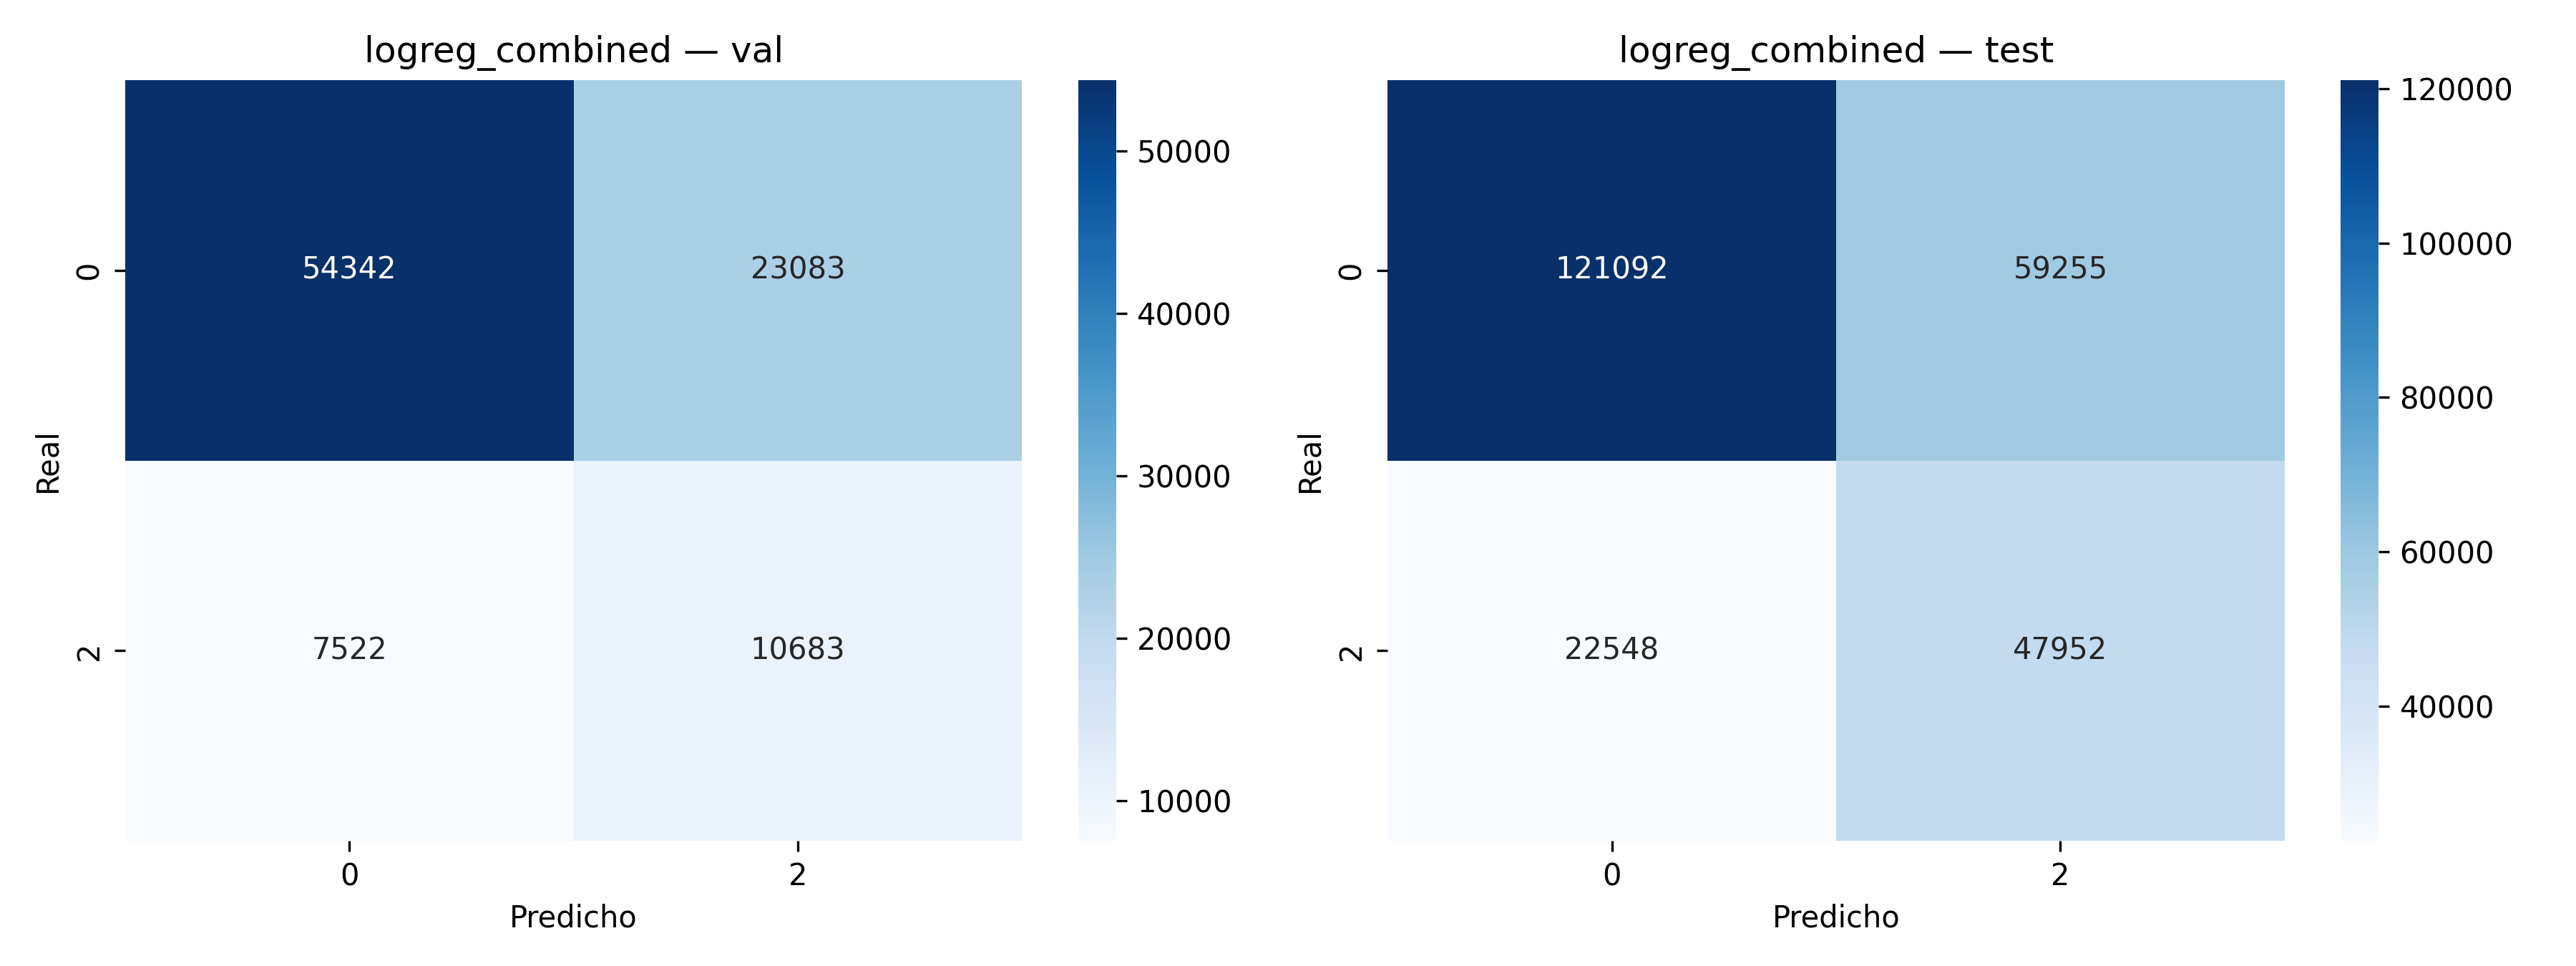
\includegraphics[width=0.9\textwidth]{combined_confusion_matrix.png}
    \caption{Matrices de confusión del modelo TF-IDF con rasgos psicolingüísticos (mono).}
    \label{fig:cm_combined}
\end{figure}

\subsection{Efecto del aumento translingüístico}
\label{sec:ablacion}
Para medir el efecto de los datos traducidos se compararon cuatro modelos con la misma configuración de submuestreo: Regresión Logística y BETO entrenados solo con datos nativos (mono) y con el corpus unificado (multi). Todos se evaluaron sobre el conjunto de prueba multi completo, desagregado por fuente (Tabla~\ref{tab:dominios} y Figura~\ref{fig:comparacion}). Para los modelos mono, las fuentes traducidas constituyen un dominio no visto durante el entrenamiento.

\begin{figure}[H]
\centering
\resizebox{\textwidth}{!}{% Diseño 2x2 (datos de entrenamiento x modelo) evaluado sobre dos dominios de prueba.
\begin{tikzpicture}[font=\footnotesize]
    % Encabezados
    \node[font=\footnotesize\bfseries, text=ugrAzul] at (-0.6, 1.25) {Datos de entrenamiento};
    \node[font=\footnotesize\bfseries, text=ugrAzul] at (3.0, 1.25) {TF-IDF + LR};
    \node[font=\footnotesize\bfseries, text=ugrAzul] at (6.0, 1.25) {BETO};

    \node[nodoES, text width=3.3cm] (dmono) at (-0.6, 0.35) {\textbf{Mono}\\ solo tweets nativos};
    \node[nodoEN, text width=3.3cm] (dmulti) at (-0.6, -1.15) {\textbf{Multi}\\ tweets nativos +\\ Reddit traducido};

    \node[proceso=2.4cm] (lrm)  at (3.0,  0.35) {LR mono};
    \node[proceso=2.4cm] (btm)  at (6.0,  0.35) {BETO mono};
    \node[proceso=2.4cm] (lrx)  at (3.0, -1.15) {LR multi};
    \node[proceso=2.4cm] (btx)  at (6.0, -1.15) {BETO multi};
    \draw[flecha] (dmono) -- (lrm);
    \draw[flecha] (dmulti) -- (lrx);

    \begin{scope}[on background layer]
        \node[draw=ugrAzul!45, dashed, rounded corners=4pt, fill=ugrAzul!3, inner sep=7pt, fit=(lrm)(btm)(lrx)(btx)] (grp) {};
    \end{scope}

    % Conjuntos de prueba
    \node[resultado=4.4cm] (tn) at (11.4, 0.35) {\textbf{Test nativo común}\\ 250\,847 tweets \textperiodcentered{} 64 usuarios};
    \node[resultado=4.4cm, draw=ugrNaranja, fill=ugrNaranja!8] (tt) at (11.4, -1.15) {\textbf{Test traducido}\\ 52\,757 textos de Reddit};
    \draw[flecha] (grp.east |- tn) -- (tn) node[midway, above, font=\scriptsize, text=ugrGris] {todos};
    \draw[flecha] (grp.east |- tt) -- (tt) node[midway, below, font=\scriptsize, text=ugrGris] {todos};
\end{tikzpicture}
}
\caption{Diseño experimental: dos modelos entrenados con dos conjuntos de datos y evaluados sobre los mismos dos dominios de prueba.}
\label{fig:diseno}
\end{figure}

\begin{table}[H]
\centering
\footnotesize
\setlength{\tabcolsep}{3.5pt}
\caption{Rendimiento por fuente del conjunto de prueba multi. F1-M: F1-macro (abreviado por espacio); Esp.: especificidad (proporción de controles bien clasificados); Exh.: exhaustividad de la clase depresiva. Reddit MH Posts solo contiene casos positivos.}
\label{tab:dominios}
\begin{tabular}{lrrrrrrrrrr}
\toprule
& \multicolumn{2}{c}{\textbf{Nativo}} & \multicolumn{3}{c}{\textbf{Kaggle SDD}} & \multicolumn{2}{c}{\textbf{Depr.\ Reddit}} & \textbf{MH Posts} & \multicolumn{2}{c}{\textbf{Total}} \\
\cmidrule(lr){2-3}\cmidrule(lr){4-6}\cmidrule(lr){7-8}\cmidrule(lr){9-9}\cmidrule(lr){10-11}
\textbf{Modelo} & F1-M & AUC & F1-M & AUC & Esp. & F1-M & AUC & Exh. & F1-M & AUC \\
\midrule
LR mono    & 0{,}653 & 0{,}753 & 0{,}418 & 0{,}802 & 0{,}085 & 0{,}574 & 0{,}906 & 0{,}900 & 0{,}657 & 0{,}769 \\
LR multi   & 0{,}648 & 0{,}719 & 0{,}834 & 0{,}962 & 0{,}704 & 0{,}758 & 0{,}911 & 0{,}856 & 0{,}704 & 0{,}787 \\
BETO mono  & \textbf{0{,}717} & \textbf{0{,}808} & 0{,}415 & 0{,}801 & 0{,}081 & 0{,}588 & 0{,}884 & \textbf{0{,}913} & 0{,}710 & 0{,}808 \\
BETO multi & 0{,}701 & 0{,}796 & \textbf{0{,}934} & \textbf{0{,}986} & \textbf{0{,}891} & \textbf{0{,}871} & \textbf{0{,}960} & 0{,}909 & \textbf{0{,}754} & \textbf{0{,}856} \\
\midrule
$n$ & \multicolumn{2}{c}{250\,847} & \multicolumn{3}{c}{46\,414} & \multicolumn{2}{c}{1\,547} & 4\,796 & \multicolumn{2}{c}{303\,604} \\
\bottomrule
\end{tabular}
\end{table}

\begin{figure}[H]
    \centering
    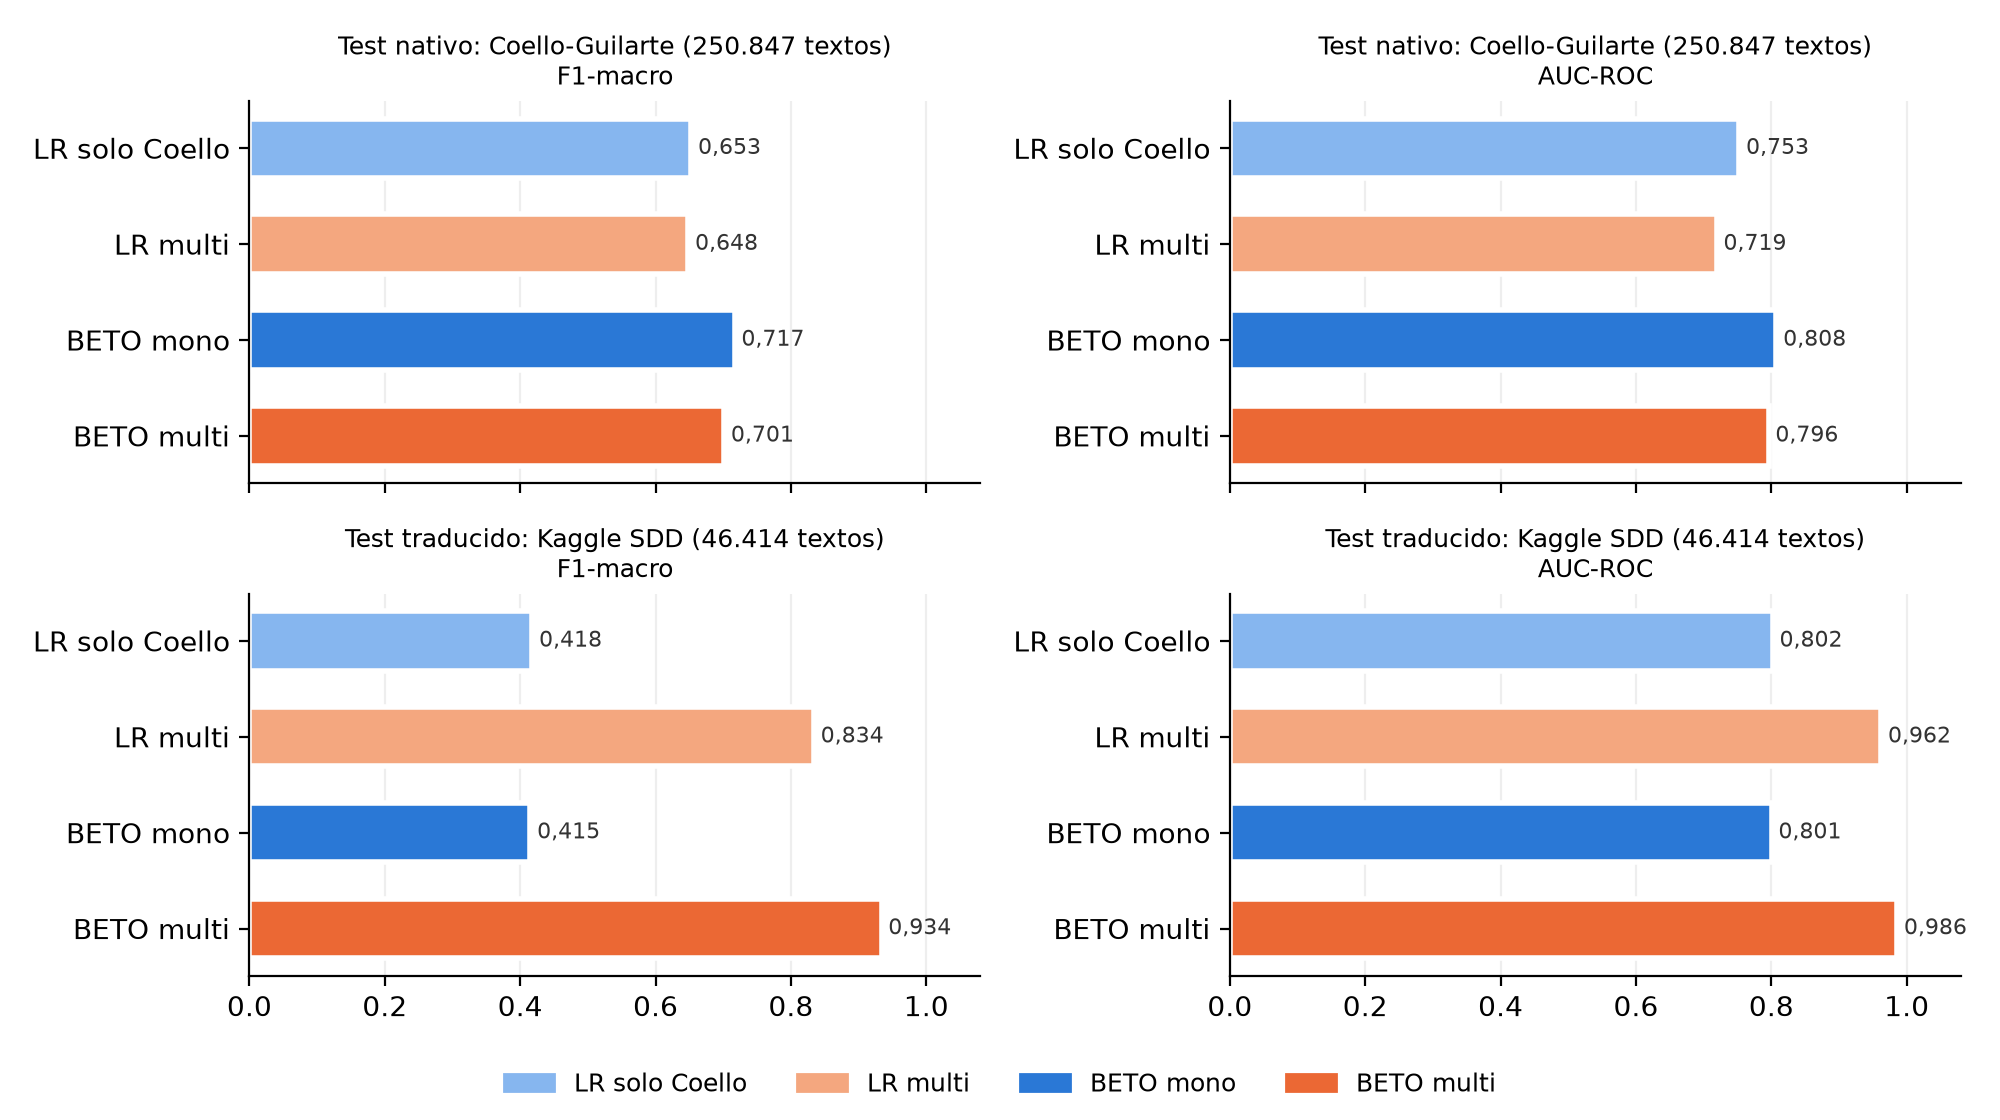
\includegraphics[width=\textwidth]{comparacion_modelos_test.png}
    \caption{F1-macro y AUC de los cuatro modelos sobre el test nativo y sobre el test traducido de Kaggle SDD.}
    \label{fig:comparacion}
\end{figure}

\begin{figure}[H]
    \centering
    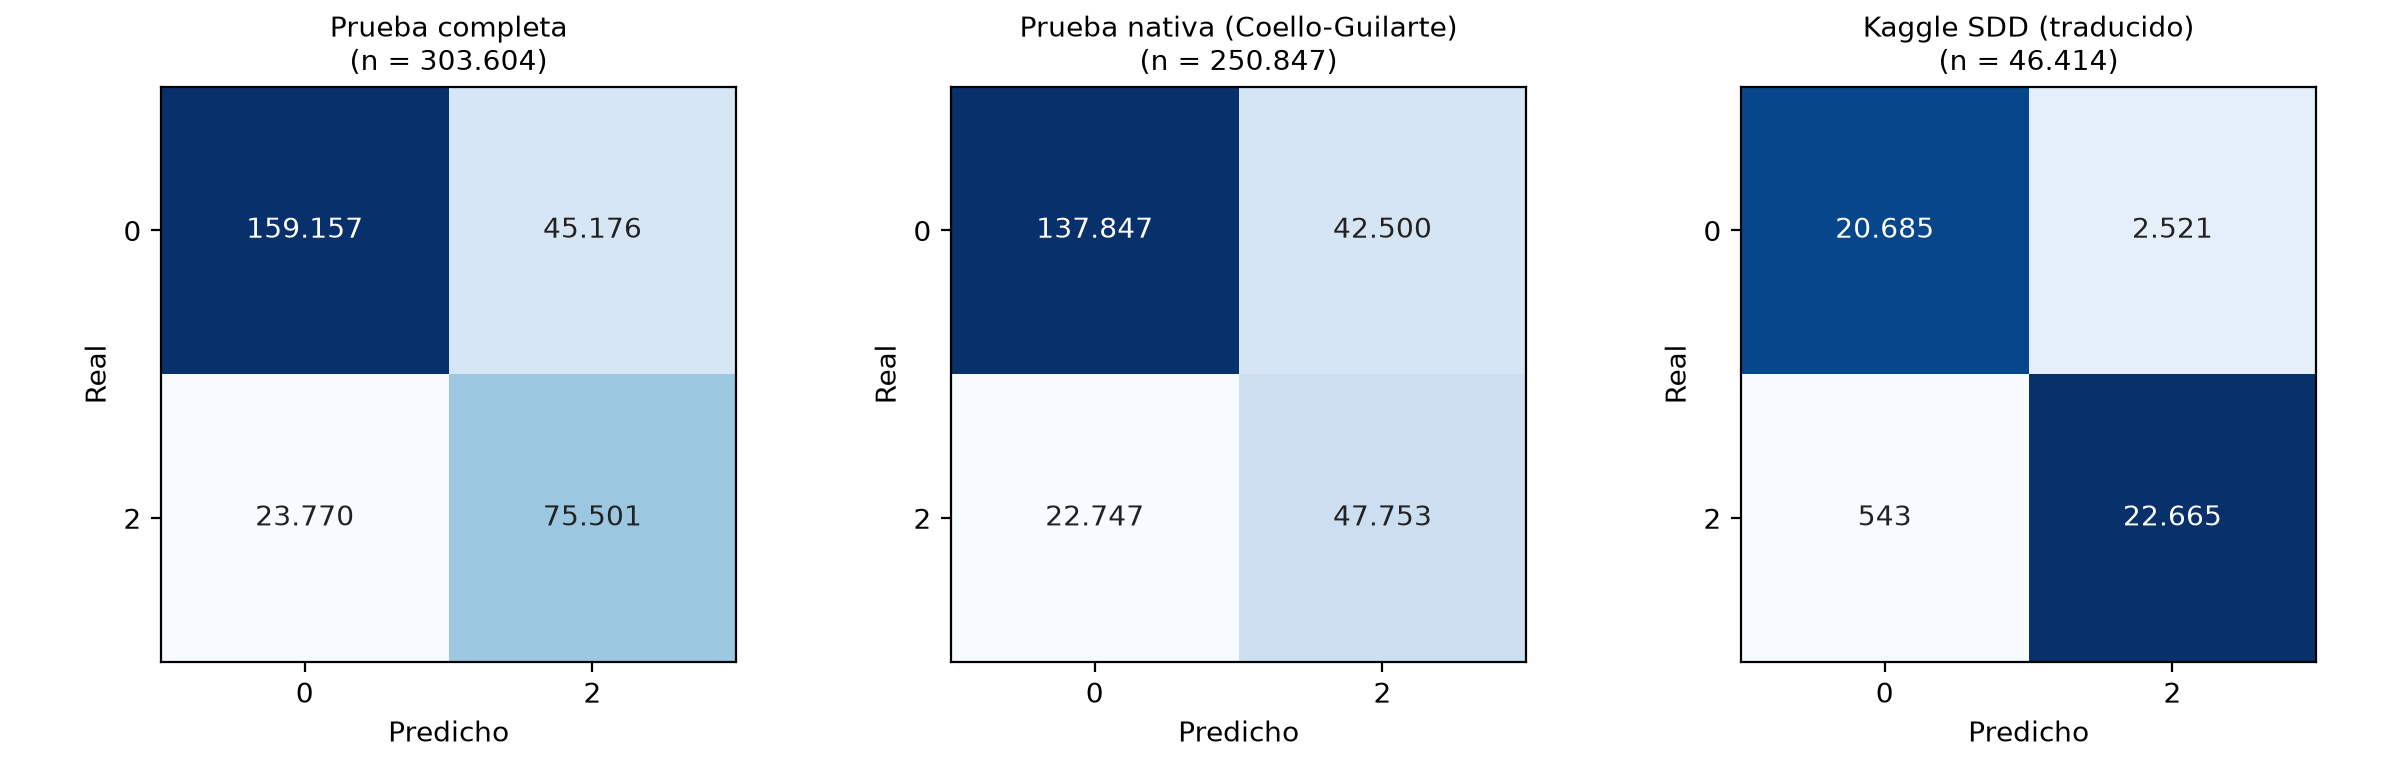
\includegraphics[width=\textwidth]{beto_multi_confusion_matrix.png}
    \caption{Matrices de confusión de BETO multi sobre el conjunto de prueba completo, la porción nativa y Kaggle SDD.}
    \label{fig:cm_beto_multi}
\end{figure}

\begin{destacado}{Hallazgo principal}
Sobre el mismo test nativo, agregar datos traducidos no mejora a ningún modelo (BETO: F1-macro 0{,}717 frente a 0{,}701). Sobre texto de Reddit, en cambio, los datos traducidos son imprescindibles (BETO: F1-macro 0{,}415 frente a 0{,}934). El aumento translingüístico amplía la cobertura de dominios, no la calidad de la detección en el dominio nativo.
\end{destacado}

Los resultados conducen a cuatro observaciones:
\begin{enumerate}[leftmargin=2em]
    \item \textbf{Los datos traducidos no mejoran la detección sobre texto nativo.} Sobre el test nativo, incorporar las traducciones reduce levemente el rendimiento de ambos modelos: la Regresión Logística pierde 0{,}4 puntos de F1-macro y 3{,}3 de AUC, y BETO pierde 1{,}6 y 1{,}2 puntos, respectivamente. En BETO la exhaustividad de la clase depresiva baja de 68{,}9\,\% a 67{,}7\,\% y la especificidad de 78{,}1\,\% a 76{,}4\,\%. Las diferencias son pequeñas, pero consistentes: en BETO empeoran las cinco métricas, y en la Regresión Logística empeoran todas salvo la exactitud, que sube porque el modelo multi clasifica más textos como control (la exhaustividad depresiva cae de 66{,}6\,\% a 51{,}1\,\%). Las diferencias pareadas (Tabla~\ref{tab:diferencias}) muestran que la degradación de BETO es pequeña pero estadísticamente distinguible de cero en F1-macro, AUC y $\kappa$, y que en la Regresión Logística la caída de AUC ($-0{,}033$) es clara mientras que la de F1-macro no lo es.
    \item \textbf{Los datos traducidos son imprescindibles para el dominio traducido.} Los modelos entrenados solo con tweets clasifican como depresivas más del 90\,\% de las publicaciones de control de Kaggle (especificidad de 0{,}08) y obtienen un F1-macro de apenas 0{,}42. Con datos traducidos en el entrenamiento, BETO multi alcanza un F1-macro de 0{,}934 y un AUC de 0{,}986 en esa fuente, y de 0{,}871 y 0{,}960 en Depression Reddit.
    \item \textbf{Indicios de un atajo de formato.} Que los modelos mono marquen como depresiva casi cualquier publicación de Reddit es coherente con lo observado en el análisis exploratorio: los textos de la clase depresiva son más largos, y una publicación de Reddit es mucho más extensa y autorreferencial que un tweet promedio. El AUC de los modelos mono en Kaggle (0{,}80) indica que conservan parte de la capacidad de ordenar los textos por riesgo, pero su umbral de decisión no se transfiere al nuevo dominio.
    \item \textbf{La métrica global depende de la mezcla de fuentes.} BETO multi obtiene el mejor F1-macro sobre el test completo (0{,}754 frente a 0{,}710 de BETO mono; diferencia pareada $+0{,}044$ con IC 95\,\% [0{,}023; 0{,}077]), pero esa ventaja proviene íntegramente de las fuentes traducidas, porque sobre la porción nativa la diferencia es negativa. Una métrica agregada sobre un conjunto de prueba multifuente no permite, por sí sola, concluir que un modelo es mejor para la población de interés.
\end{enumerate}

En consecuencia, \Hs{1} no se sostiene para el texto nativo: el aumento translingüístico, tal como se implementó, amplía los dominios en los que el modelo funciona, pero no mejora la detección sobre tweets en español. Dos factores pueden explicarlo. Por un lado, los textos traducidos difieren de los tweets en plataforma, longitud y registro, de modo que lo que el modelo aprende de ellos se transfiere poco al dominio nativo. Por otro, la selección del mejor punto de control de BETO multi se hizo sobre un conjunto de validación mixto (78\,\% nativo), que no optimiza exclusivamente el rendimiento nativo.

\subsection{Interpretabilidad: ¿qué aprende el modelo léxico?}
Se analizaron los 15 términos con mayor coeficiente hacia cada clase en la Regresión Logística mono. Los asociados a la clase depresiva son, mayoritariamente, marcadores dialectales o geográficos: formas propias del español peninsular (\emph{os}, \emph{tenéis}, \emph{joder}, \emph{gilipollas}), del rioplatense (\emph{vos}, \emph{ahre}), referencias a política y países de Sudamérica (\emph{piñera}, \emph{uribe}, \emph{colombia}, \emph{venezuela}) y términos de comunidades en línea (\emph{hilo}, \emph{army}). Los asociados a la clase control son marcadores del español mexicano (\emph{wey}, \emph{mexicanos}, \emph{puebla}, \emph{colima}, \emph{chihuahua}, \emph{veracruz}, \emph{tigres}, \emph{gobernador}) y de la vida escolar (\emph{tarea}, \emph{semestre}).

Ninguno de los treinta términos extremos corresponde a los marcadores psicolingüísticos descritos en la literatura. El patrón indica que, en este corpus, la etiqueta está fuertemente asociada a la procedencia geográfica del usuario: los controles son mayoritariamente usuarios mexicanos y los usuarios depresivos provienen con mayor frecuencia de otros países hispanohablantes. El modelo léxico explota esa correlación, un caso de aprendizaje por atajos~\cite{geirhos2020shortcut}. Como la partición es por usuario, el atajo se generaliza al conjunto de prueba (que tiene la misma composición geográfica), de modo que las métricas no lo penalizan; pero un modelo así fallaría al aplicarse, por ejemplo, a una población rioplatense, donde todo usuario usaría \emph{vos}.

\paragraph{Contraste con el lexicón psicolingüístico.} Que los marcadores clínicos no figuren entre los términos extremos no implica que el modelo los ignore. Para contrastar \Hs{3} de forma sistemática se ubicó cada término del lexicón dentro de la distribución completa de coeficientes (Tabla~\ref{tab:hs4}). Las emociones negativas son la única categoría con un sesgo claro hacia la clase depresiva: 21 de sus 22 términos presentes en el vocabulario tienen coeficiente positivo, entre ellos \emph{morirme}, \emph{suicidio}, \emph{vacío}, \emph{deprimido} y \emph{tristeza}, y seis aparecen entre los 500 unigramas más asociados a la clase depresiva (Fisher, $p=0{,}003$). Las emociones positivas se inclinan, como se esperaba, hacia la clase control. En cambio, la primera persona del singular y el lenguaje absolutista no se distinguen del resto del vocabulario ($p>0{,}09$), en coherencia con el análisis exploratorio (Tabla~\ref{tab:marcadores}). En el modelo con submuestreo el patrón es el mismo, aunque la concentración de emociones negativas en el extremo superior es menos marcada (Fisher, $p=0{,}08$; Mann-Whitney, $p<0{,}001$).

\begin{table}[H]
\centering
\footnotesize
\setlength{\tabcolsep}{4pt}
\caption{Términos del lexicón psicolingüístico en la Regresión Logística mono (ponderación). Top-500: unigramas con mayor coeficiente depresivo entre 15\,000 términos del vocabulario.}
\label{tab:hs4}
\begin{tabular}{lrrrrr}
\toprule
\textbf{Categoría} & \textbf{En vocab.} & \textbf{Coef. $>0$} & \textbf{En top-500} & \textbf{$p$ Fisher} & \textbf{$p$ Mann-Whitney} \\
\midrule
Primera persona singular & 7  & 57\,\% & 1 & 0{,}40 & 0{,}093 \\
Absolutistas             & 9  & 78\,\% & 0 & 1{,}00 & 0{,}094 \\
Emoción negativa         & 22 & 95\,\% & 6 & 0{,}003 & $<0{,}001$ \\
Emoción positiva         & 18 & 22\,\% & 1 & 0{,}73 & 0{,}98 \\
\bottomrule
\end{tabular}

\vspace{0.15cm}
{\footnotesize Ambas pruebas son unilaterales (mayor asociación con la clase depresiva). Para la emoción positiva, un valor de $p$ alto es el resultado esperado.}
\end{table}

\subsection{Control experimental del atajo dialectal}
\label{sec:control_dialectal}
La Tabla~\ref{tab:control_dialecto} muestra el efecto de enmascarar los marcadores diatópicos sobre el test nativo, según el protocolo de la Sección~\ref{sec:met_dialecto}.

\begin{table}[H]
\centering
\footnotesize
\setlength{\tabcolsep}{4pt}
\caption{Efecto del enmascarado de marcadores diatópicos sobre el test nativo. Diferencias respecto del texto original con IC 95\,\% por \emph{bootstrap} de usuarios.}
\label{tab:control_dialecto}
\begin{tabular}{llccc}
\toprule
\textbf{Modelo} & \textbf{Condición} & \textbf{F1-macro} & \textbf{$\Delta$ F1-macro} & \textbf{$\Delta$ AUC} \\
\midrule
\multirow{6}{*}{LR mono}
 & Original              & 0{,}655 & -- & -- \\
 & Dialectismos          & 0{,}648 & $-0{,}007$ {\scriptsize [$-0{,}010$; $-0{,}004$]} & $-0{,}010$ {\scriptsize [$-0{,}014$; $-0{,}006$]} \\
 & Topónimos             & 0{,}648 & $-0{,}007$ {\scriptsize [$-0{,}015$; $-0{,}003$]} & $-0{,}012$ {\scriptsize [$-0{,}026$; $-0{,}003$]} \\
 & Figuras políticas     & 0{,}654 & $-0{,}001$ {\scriptsize [$-0{,}003$; $-0{,}000$]} & $-0{,}002$ {\scriptsize [$-0{,}005$; $-0{,}000$]} \\
 & Todos                 & 0{,}640 & $-0{,}015$ {\scriptsize [$-0{,}025$; $-0{,}009$]} & $-0{,}025$ {\scriptsize [$-0{,}042$; $-0{,}013$]} \\
 & Control aleatorio     & 0{,}655 & $\phantom{-}0{,}000$ {\scriptsize [$-0{,}000$; 0{,}000]} & $\phantom{-}0{,}000$ {\scriptsize [$-0{,}000$; 0{,}000]} \\
\midrule
\multirow{3}{*}{SVM mono}
 & Original              & 0{,}653 & -- & -- \\
 & Todos                 & 0{,}639 & $-0{,}015$ {\scriptsize [$-0{,}024$; $-0{,}008$]} & $-0{,}024$ {\scriptsize [$-0{,}039$; $-0{,}013$]} \\
 & Control aleatorio     & 0{,}653 & $\phantom{-}0{,}000$ {\scriptsize [$-0{,}000$; 0{,}000]} & $\phantom{-}0{,}000$ {\scriptsize [$-0{,}000$; 0{,}000]} \\
\midrule
\multirow{3}{*}{BETO mono}
 & Original              & 0{,}717 & -- & -- \\
 & Todos                 & 0{,}703 & $-0{,}014$ {\scriptsize [$-0{,}024$; $-0{,}008$]} & $-0{,}021$ {\scriptsize [$-0{,}034$; $-0{,}011$]} \\
 & Control aleatorio     & 0{,}717 & $-0{,}0001$ {\scriptsize [$-0{,}0005$; 0{,}0002]} & $-0{,}0003$ {\scriptsize [$-0{,}0006$; $-0{,}0001$]} \\
\midrule
\multirow{3}{*}{BETO multi}
 & Original              & 0{,}701 & -- & -- \\
 & Todos                 & 0{,}687 & $-0{,}014$ {\scriptsize [$-0{,}024$; $-0{,}008$]} & $-0{,}020$ {\scriptsize [$-0{,}033$; $-0{,}011$]} \\
 & Control aleatorio     & 0{,}701 & $-0{,}0002$ {\scriptsize [$-0{,}0007$; 0{,}0001]} & $-0{,}0005$ {\scriptsize [$-0{,}0009$; $-0{,}0000$]} \\
\bottomrule
\end{tabular}
\end{table}

Los resultados permiten tres conclusiones:
\begin{enumerate}[leftmargin=2em]
    \item \textbf{Los marcadores regionales tienen un efecto propio.} Aunque solo el 7{,}9\,\% de los tweets contiene algún marcador, enmascararlos reduce el F1-macro de todos los modelos en unos 1{,}5 puntos y el AUC en 2 a 2{,}5 puntos, con intervalos que excluyen el cero. Enmascarar la misma cantidad de palabras elegidas al azar produce cambios al menos cuarenta veces menores (como máximo 0{,}0005 de AUC, en BETO), de modo que la caída se debe al contenido regional de esas palabras y no a la pérdida de texto.
    \item \textbf{BETO también utiliza el atajo.} La caída de BETO es prácticamente igual a la de los modelos léxicos. La prueba responde así la pregunta que el análisis de coeficientes dejaba abierta: el modelo contextual no evita el atajo dialectal.
    \item \textbf{El atajo no explica la ventaja de BETO.} Con los marcadores enmascarados, BETO mono (0{,}703) sigue superando a la Regresión Logística (0{,}640) por un margen similar al original, porque ambos modelos pierden lo mismo.
\end{enumerate}
La magnitud medida es una cota inferior del efecto regional. El lexicón se construyó a partir de los coeficientes de la Regresión Logística (calculados sobre el entrenamiento), lo que podría favorecer una caída mayor en ese modelo; que BETO pierda lo mismo refuerza la conclusión de que también depende de esos términos. El lexicón solo cubre los marcadores explícitos más frecuentes, y los usuarios de cada región difieren también en temas, registro y estilo, señales que el enmascarado no elimina. Un modelo reentrenado sin estos términos, por otra parte, podría compensar con otras señales correlacionadas con la región. Como el 92\,\% de los tweets no contiene ningún marcador, el efecto por tweet afectado es considerable aunque la caída global sea moderada.

\subsection{Contraste de hipótesis}
\begin{table}[H]
\centering
\small
\caption{Síntesis del contraste de hipótesis.}
\label{tab:hipotesis}
\begin{tabularx}{\textwidth}{lp{2.4cm}X}
\toprule
\textbf{Hipótesis} & \textbf{Resultado} & \textbf{Evidencia} \\
\midrule
Principal & Sostenida a nivel de documento & Sobre el test nativo común, BETO supera a la Regresión Logística y a la SVM sobre TF-IDF en F1-macro, F1 depresivo, AUC y $\kappa$ (F1-macro 0{,}717 frente a 0{,}655; AUC 0{,}808 frente a 0{,}755), tanto con datos mono como multi, con diferencias pareadas cuyos intervalos del 95\,\% excluyen el cero (Tabla~\ref{tab:diferencias}); también lo supera en las fuentes traducidas cuando ambos se entrenan con datos multi. La ventaja no proviene del atajo dialectal, que afecta por igual a ambos modelos. Fuera de su dominio de entrenamiento, ninguno de los dos modelos funciona, y al agregar las predicciones por usuario la ventaja desaparece (Sección~\ref{sec:res_usuario}). \\
\addlinespace
\Hs{1} Aumento translingüístico & No sostenida para texto nativo & Con datos traducidos, el rendimiento sobre tweets nativos baja levemente en ambos modelos (BETO: 0{,}717 a 0{,}701 de F1-macro; diferencia pareada $-0{,}016$, IC 95\,\% [$-0{,}035$; $-0{,}004$]). Las traducciones sí son necesarias para clasificar texto del dominio traducido (Sección~\ref{sec:ablacion}). \\
\addlinespace
\Hs{2} Rasgos psicolingüísticos & No sostenida & El modelo combinado no mejora a TF-IDF solo (F1-macro 0{,}644 frente a 0{,}653). Esta diferencia no se acompañó de intervalo de confianza porque el modelo requiere recalcular sus rasgos temporales. \\
\addlinespace
\Hs{3} Consistencia psicolingüística & Sostenida parcialmente & En la Regresión Logística, los términos de emoción negativa se concentran en el extremo depresivo de los coeficientes (Fisher $p=0{,}003$) y los de emoción positiva en el de control, pero la primera persona y el absolutismo no se distinguen del resto del vocabulario. Los términos de mayor peso son dialectales y geográficos. \\
\bottomrule
\end{tabularx}
\end{table}

\subsection{Análisis de errores}
En el escenario mono, BETO produce 39\,497 falsos positivos y 21\,915 falsos negativos en prueba. Dos factores estructurales explican buena parte de esos errores:
\begin{itemize}[leftmargin=2em]
    \item \textbf{Etiqueta por usuario, predicción por texto.} Todos los tweets de un usuario depresivo heredan la etiqueta positiva, aunque la mayoría trate temas cotidianos (deporte, política, saludos). Un tweet como ``JAJAJA'' o ``¡Pregúntame cualquier cosa!'' no contiene información sobre el estado de ánimo, y su clasificación es necesariamente cercana al azar. Esto pone un techo bajo al rendimiento por documento.
    \item \textbf{Textos muy cortos.} Con una mediana de 10 tokens, muchos tweets no contienen ningún marcador lingüístico relevante.
\end{itemize}
Desde la perspectiva del cribado, un falso negativo deja sin orientación a una persona en riesgo, mientras que un falso positivo, en un sistema que solo ofrece información sobre recursos de ayuda, tiene un costo menor. Por ello resulta preferible operar con umbrales que favorezcan la exhaustividad de la clase depresiva. Sin embargo, un falso positivo no es inocuo: rotular a una persona como posible caso de depresión tiene implicancias de estigmatización y privacidad que deben considerarse en cualquier despliegue.

\subsection{Evaluación a nivel de usuario}
\label{sec:res_usuario}
Agregar las predicciones por usuario (Sección~\ref{sec:met_usuario}) mitiga ambos factores y acerca la tarea a su formulación clínica, en la que se evalúa a la persona y no a un mensaje aislado. La Tabla~\ref{tab:usuario} muestra el resultado sobre los 64 usuarios del test nativo.

\begin{table}[H]
\centering
\footnotesize
\setlength{\tabcolsep}{4pt}
\caption{Métricas a nivel de usuario sobre el test nativo (64 usuarios, 19 depresivos), agregando el score medio de cada usuario. IC 95\,\% por \emph{bootstrap} de usuarios.}
\label{tab:usuario}
\begin{tabular}{lccc}
\toprule
\textbf{Modelo} & \textbf{F1-macro} & \textbf{AUC} & \textbf{$\kappa$} \\
\midrule
LR mono (ponderación) & 0{,}925 {\scriptsize [0{,}845; 0{,}982]} & 0{,}989 {\scriptsize [0{,}968; 1{,}000]} & 0{,}850 {\scriptsize [0{,}691; 0{,}963]} \\
SVM mono              & 0{,}943 {\scriptsize [0{,}867; 1{,}000]} & 0{,}989 {\scriptsize [0{,}967; 1{,}000]} & 0{,}886 {\scriptsize [0{,}734; 1{,}000]} \\
BETO mono             & 0{,}888 {\scriptsize [0{,}800; 0{,}964]} & 0{,}982 {\scriptsize [0{,}954; 0{,}999]} & 0{,}775 {\scriptsize [0{,}601; 0{,}927]} \\
LR multi              & 0{,}875 {\scriptsize [0{,}771; 0{,}961]} & 0{,}988 {\scriptsize [0{,}965; 1{,}000]} & 0{,}753 {\scriptsize [0{,}559; 0{,}923]} \\
BETO multi            & 0{,}884 {\scriptsize [0{,}791; 0{,}963]} & 0{,}978 {\scriptsize [0{,}944; 0{,}998]} & 0{,}768 {\scriptsize [0{,}582; 0{,}925]} \\
\bottomrule
\end{tabular}
\end{table}

Al pasar del tweet al usuario el AUC sube de 0{,}72--0{,}81 a 0{,}98--0{,}99 en todos los modelos: la señal acumulada en miles de tweets por usuario separa casi perfectamente ambos grupos. Dos observaciones limitan la lectura de este resultado. Primero, la ventaja de BETO desaparece: a nivel de usuario los modelos léxicos obtienen valores iguales o superiores, con intervalos ampliamente superpuestos, de modo que con 64 usuarios no es posible ordenar los modelos. Segundo, repetir la agregación sobre las predicciones con los marcadores enmascarados apenas modifica la separación: el AUC por usuario pasa de 0{,}989 a 0{,}986 en la Regresión Logística y de 0{,}982 a 0{,}972 en BETO mono, y el F1-macro baja entre 0 y 5{,}5 puntos según el modelo (uno o dos usuarios cambian de clase). Los marcadores explícitos no son, entonces, los que sostienen la separación por usuario, pero eso no permite atribuirla a señales clínicas: con miles de tweets por persona también se acumulan señales regionales indirectas (temas, registro, actualidad local) que el lexicón no cubre. El rendimiento casi perfecto a nivel de usuario debe leerse como evidencia de que ambos grupos de usuarios del corpus son altamente distinguibles, no como una estimación de la capacidad de detectar depresión en una población nueva. La agregación por proporción de tweets positivos produce resultados equivalentes (tabla completa en \texttt{informe/tables/user\_level\_metrics.csv}).

\subsection{Variación dialectal}
El español presenta una variación diatópica considerable. Los resultados de este trabajo muestran que esa variación no es un detalle menor sino una fuente de sesgo de primer orden:
\begin{itemize}[leftmargin=2em]
    \item El corpus nativo combina variedades (mexicana, peninsular, rioplatense, andina) con una distribución desigual entre clases, y tanto los modelos léxicos como BETO aprenden esa desigualdad (Sección~\ref{sec:control_dialectal}).
    \item La traducción automática produce un registro relativamente uniforme con rasgos peninsulares (\emph{tienes}, \emph{me he}), que difiere del registro de los tweets nativos. Si una fuente traducida se concentra en una clase, el registro de traducción puede convertirse a su vez en un atajo.
    \item La tokenización por subpalabras de BETO reduce el problema de palabras fuera de vocabulario ante variantes como \emph{querés} y \emph{quieres}, pero no elimina la posibilidad de que el modelo asocie esas variantes a una clase.
\end{itemize}
Un corpus balanceado por región (rioplatense, andina, centroamericana, caribeña, mexicana y peninsular) y una evaluación desagregada por variedad son requisitos para una herramienta aplicable en Argentina o en cualquier otro país hispanohablante.

\subsection{Limitaciones y amenazas a la validez}
\paragraph{Validez de constructo.} Las etiquetas no provienen de diagnósticos clínicos sino de la clasificación de usuarios en el corpus original y de la pertenencia a comunidades de Reddit. Publicar en \texttt{r/depression} no equivale a padecer depresión, y publicar en \texttt{r/teenagers} no excluye padecerla. En Kaggle SDD, además, la clase positiva incluye \texttt{r/SuicideWatch}, que corresponde a un constructo distinto (ideación suicida).

\paragraph{Validez interna.} La correlación entre etiqueta y procedencia geográfica en Coello-Guilarte es un factor de confusión que afecta a todos los modelos; el control experimental la cuantificó para los marcadores explícitos, pero no puede eliminar las señales regionales indirectas (temas, registro). En las fuentes traducidas, la clase está asociada a la comunidad de origen (\texttt{r/teenagers} frente a \texttt{r/depression}), por lo que el alto rendimiento sobre esas fuentes puede reflejar en parte la distinción temática entre comunidades más que la sintomatología. Por último, Kaggle SDD no tiene autor, de modo que se trató cada publicación como un usuario; si un mismo autor publicó varias veces, sus textos pueden haber quedado en particiones distintas, lo que podría sobrestimar levemente el rendimiento en esa fuente.

\paragraph{Validez externa.} Los modelos se entrenaron con tweets de un período y una población determinados y con publicaciones de Reddit traducidas. No hay evidencia de que generalicen a otras plataformas (WhatsApp, Instagram, Telegram), a otras variedades del español ni a textos de otro período~\cite{harrigian2020generalize}. Los resultados de la Sección~\ref{sec:ablacion} muestran, de hecho, que un modelo entrenado en un dominio puede fallar de forma sistemática en otro.

\paragraph{Validez estadística.} Cada modelo se entrenó una sola vez con una semilla fija y se evaluó sobre una única partición. Los intervalos por \emph{bootstrap} de usuarios cuantifican la incertidumbre debida a la muestra de 64 usuarios de prueba, pero no la variabilidad debida a la semilla de entrenamiento ni a la asignación de usuarios entre particiones, que requeriría reentrenar. Las diferencias pequeñas, como la de BETO mono frente a multi en el test nativo ($-0{,}016$ de F1-macro), son distinguibles de cero dentro de esta partición, pero no puede descartarse que cambien de signo con otra semilla o partición. A nivel de usuario, con 19 casos positivos, la potencia es insuficiente para comparar modelos.

\paragraph{Reproducibilidad.} Los pesos de los modelos, las predicciones de prueba y los manifiestos se conservan localmente; los corpus de origen se distribuyen bajo licencias de investigación y no se redistribuyen.

\subsection{Consideraciones éticas}
Se siguieron las recomendaciones de la literatura sobre investigación en salud mental digital~\cite{fisher2025metaanalisis,leis2021tesis}:
\begin{itemize}[leftmargin=2em]
    \item uso exclusivo de datos públicos y anonimización previa a cualquier análisis;
    \item ausencia de intento de reidentificación de usuarios;
    \item transparencia sobre las limitaciones y sesgos detectados;
    \item declaración explícita de que el sistema \emph{no} diagnostica y \emph{no} reemplaza la evaluación profesional.
\end{itemize}
Cualquier aplicación práctica requeriría validación con profesionales de la salud mental, consentimiento informado de los usuarios, mecanismos de exclusión voluntaria, auditoría de sesgos por región, género y edad, y un protocolo de derivación a servicios de ayuda. El monitoreo automático de personas sin su consentimiento no es un uso aceptable de esta tecnología.

\newpage
% =====================================================================
% 6. CONCLUSIONES
% =====================================================================
\section{Conclusiones y trabajo futuro}
\label{sec:conclusiones}

\subsection{Conclusiones}
\begin{enumerate}[leftmargin=2em]
    \item \textbf{El modelo contextual en español supera a los modelos léxicos a nivel de publicación.} Sobre el test nativo común, BETO mejora a TF-IDF con Regresión Logística y con SVM en todas las métricas, con ganancias de 5 a 6 puntos de F1-macro y de 5 a 8 puntos de AUC según los datos de entrenamiento, y con diferencias pareadas cuyos intervalos del 95\,\% por \emph{bootstrap} de usuarios excluyen el cero. El mejor modelo para texto nativo, BETO mono, alcanza un F1-macro de 0{,}717 (IC 95\,\%: 0{,}665--0{,}759), un AUC de 0{,}808 y una exhaustividad del 69\,\% en la clase depresiva. Al agregar las predicciones por usuario todos los modelos separan casi perfectamente a los 64 usuarios de prueba (AUC $\geq 0{,}97$) y la ventaja de BETO deja de observarse.
    \item \textbf{El aumento translingüístico amplía la cobertura, pero no mejora el dominio nativo.} Incorporar 263\,829 publicaciones de Reddit traducidas no mejoró la detección sobre tweets en español (BETO: 0{,}717 frente a 0{,}701 de F1-macro), pero permitió que el modelo funcionara sobre el dominio traducido, donde los modelos mono fallan de forma sistemática (F1-macro de 0{,}93 frente a 0{,}42 en Kaggle SDD).
    \item \textbf{La evaluación de corpus multifuente requiere particiones y métricas por fuente.} Una primera versión de las particiones sobrestimó el efecto del aumento por la forma en que una fuente sin autores fue asignada a entrenamiento y prueba. Incluso con particiones correctas, la métrica global sobre un test mezclado favorece al modelo multi por razones que no se relacionan con la población de interés. La auditoría sistemática de las particiones y la evaluación desagregada fueron decisivas para llegar a conclusiones válidas.
    \item \textbf{Todos los modelos, incluido BETO, aprenden atajos dialectales.} Los términos más predictivos del modelo léxico son marcadores de procedencia geográfica y no marcadores clínicos. Enmascarar 175 marcadores regionales, presentes en solo el 7{,}9\,\% de los tweets, reduce el F1-macro de todos los modelos en unos 1{,}5 puntos y el AUC en 2 a 2{,}5 puntos, mientras que enmascarar la misma cantidad de palabras al azar no tiene efecto apreciable. BETO pierde lo mismo que los modelos léxicos, por lo que el atajo no explica su ventaja, pero tampoco la evita. Los modelos entrenados solo con tweets muestran además indicios de un atajo de longitud o formato. Estos resultados solo fueron visibles gracias al análisis de interpretabilidad, al control experimental y a la evaluación fuera de dominio, lo que confirma su valor como herramientas de auditoría.
    \item \textbf{Los marcadores psicolingüísticos se reflejan solo en parte en el modelo lineal y no aportan como rasgos explícitos.} En la Regresión Logística, los términos de emoción negativa se concentran en el extremo depresivo de los coeficientes y los de emoción positiva en el de control, pero la primera persona y el lenguaje absolutista no se distinguen del resto del vocabulario. Incorporar esos marcadores como rasgos explícitos no mejora el rendimiento.
    \item \textbf{Interpretabilidad y replicabilidad.} La interpretabilidad se alcanzó a nivel global para los modelos lineales y como auditoría de atajos para todos los modelos; la interpretabilidad \emph{post hoc} de BETO queda pendiente. El pipeline completo (descarga, anonimización, traducción, unificación, partición, modelado y evaluación) está automatizado con semillas fijas, configuraciones versionadas, manifiestos y un registro único de métricas, y todas las métricas, intervalos y controles del Capítulo~\ref{sec:resultados} se recalculan con un único comando a partir de las predicciones guardadas. La reproducción exacta de la línea base mono a partir del esquema multi y de las métricas originales a partir de los modelos guardados lo confirma.
\end{enumerate}

\subsection{Trabajo futuro}
\begin{itemize}[leftmargin=2em]
    \item \textbf{Control del sesgo geográfico.} Reentrenar los modelos sobre texto con los marcadores dialectales enmascarados, para estimar el rendimiento de un modelo que no puede usarlos; construir o filtrar un subconjunto balanceado por país y evaluar por variedad.
    \item \textbf{Aumento orientado al dominio nativo.} Probar estrategias que aprovechen los datos traducidos sin degradar el dominio nativo: preentrenamiento adicional sobre el texto traducido seguido de ajuste fino solo con tweets, ponderación por fuente o selección del modelo con validación exclusivamente nativa.
    \item \textbf{Detección temprana a nivel de usuario.} Extender la agregación por usuario a ventanas temporales y a decisiones secuenciales, en línea con el protocolo de detección temprana de eRisk, sobre un corpus con más usuarios de prueba.
    \item \textbf{Explicabilidad de BETO.} Aplicar SHAP y LIME, y análisis de atención, para verificar si el modelo contextual utiliza marcadores clínicos o atajos.
    \item \textbf{Corpus anotados clínicamente.} Gestionar el acceso a MentalRiskES y al corpus de Leis et al., y explorar colaboraciones con profesionales para obtener etiquetas basadas en instrumentos validados (PHQ-9).
    \item \textbf{Otros modelos.} Comparar con modelos multilingües (XLM-RoBERTa), con modelos en español más recientes (RoBERTa-BNE, MarIA) y con modelos generativos ajustados por instrucciones.
    \item \textbf{Variabilidad de entrenamiento.} Complementar los intervalos por \emph{bootstrap} de usuarios repitiendo los entrenamientos con varias semillas y particiones.
\end{itemize}

\newpage
% =====================================================================
% BIBLIOGRAFÍA
% =====================================================================
\bibliographystyle{ieeetr}
\bibliography{references}

\newpage
% =====================================================================
% ANEXOS
% =====================================================================
\appendix
\section{Anexos}

\subsection{Reproducción del pipeline}
\label{anx:reproduccion}
El repositorio expone un objetivo de \texttt{make} por etapa. La secuencia para reproducir los resultados es:

\begin{lstlisting}
make setup                 # entorno virtual y dependencias
make data                  # descarga, limpieza, unificacion y particion
python -m src.data.project_user_csvs
make translate SOURCE=kaggle_sdd BACKEND=opus_mt
make translate SOURCE=reddit_mh_posts BACKEND=opus_mt
make translate SOURCE=depression_reddit BACKEND=opus_mt
python -m src.data.merge_corpora
python -m src.data.build_splits --out ./data/processed/splits_multi
make eda                   # notebooks de analisis exploratorio
make baseline              # TF-IDF + LR / SVM (mono)
python temp/ablation_per_source.py   # TF-IDF + LR (multi y solo nativo)
make beto-multi            # ajuste fino de BETO (multi, GPU)
make eval-beto-multi       # evaluacion de BETO multi en val y test
make test                  # pruebas automaticas
# Validacion sin reentrenar (Capitulo 5)
python -m src.evaluation.run_validation          # IC, diferencias, Hs3, usuario
python -m src.evaluation.dialect_control --beto  # control dialectal (GPU)
\end{lstlisting}

Los modelos mono de BETO y el modelo combinado se entrenan a partir de los cuadernos ubicados en \path{notebooks/04_beto/02_finetune_beto_local.ipynb} y \path{notebooks/03_baseline/03_combined_features.ipynb}; sus copias ejecutadas se conservan en \texttt{reports/}.

\subsection{Manifiestos de las particiones}
\label{anx:manifiestos}

\begin{table}[H]
\centering
\small
\caption{Composición de \texttt{splits\_multi} por fuente y clase (filas).}
\label{tab:manifiesto_multi}
\begin{tabular}{llrrr}
\toprule
\textbf{Fuente} & \textbf{Clase} & \textbf{Entrenamiento} & \textbf{Validación} & \textbf{Prueba} \\
\midrule
\multirow{2}{*}{Coello-Guilarte}   & 0 & 488\,499 & 77\,425 & 180\,347 \\
                                   & 2 & 212\,218 & 18\,205 &  70\,500 \\
\multirow{2}{*}{Kaggle SDD}        & 0 &  81\,222 & 11\,603 &  23\,206 \\
                                   & 2 &  81\,224 & 11\,604 &  23\,208 \\
Reddit MH Posts                    & 2 &  16\,808 &  2\,427 &   4\,796 \\
\multirow{2}{*}{Depression Reddit} & 0 &   2\,729 &     391 &      780 \\
                                   & 2 &   2\,681 &     383 &      767 \\
\midrule
\multicolumn{2}{l}{\textbf{Total}} & \textbf{885\,381} & \textbf{122\,038} & \textbf{303\,604} \\
\bottomrule
\end{tabular}
\end{table}

\begin{table}[H]
\centering
\small
\caption{Usuarios por fuente y partición en \texttt{splits\_multi}. En Kaggle SDD y Depression Reddit cada publicación es un usuario sintético.}
\label{tab:usuarios_multi}
\begin{tabular}{lrrr}
\toprule
\textbf{Fuente} & \textbf{Entrenamiento} & \textbf{Validación} & \textbf{Prueba} \\
\midrule
Coello-Guilarte   &      221 &     32 &      64 \\
Kaggle SDD        & 162\,446 & 23\,207 & 46\,414 \\
Reddit MH Posts   &  14\,168 &  2\,025 &  4\,049 \\
Depression Reddit &   5\,410 &    774 &  1\,547 \\
\bottomrule
\end{tabular}
\end{table}

\subsection{Matrices de confusión de la línea base}

\begin{figure}[H]
    \centering
    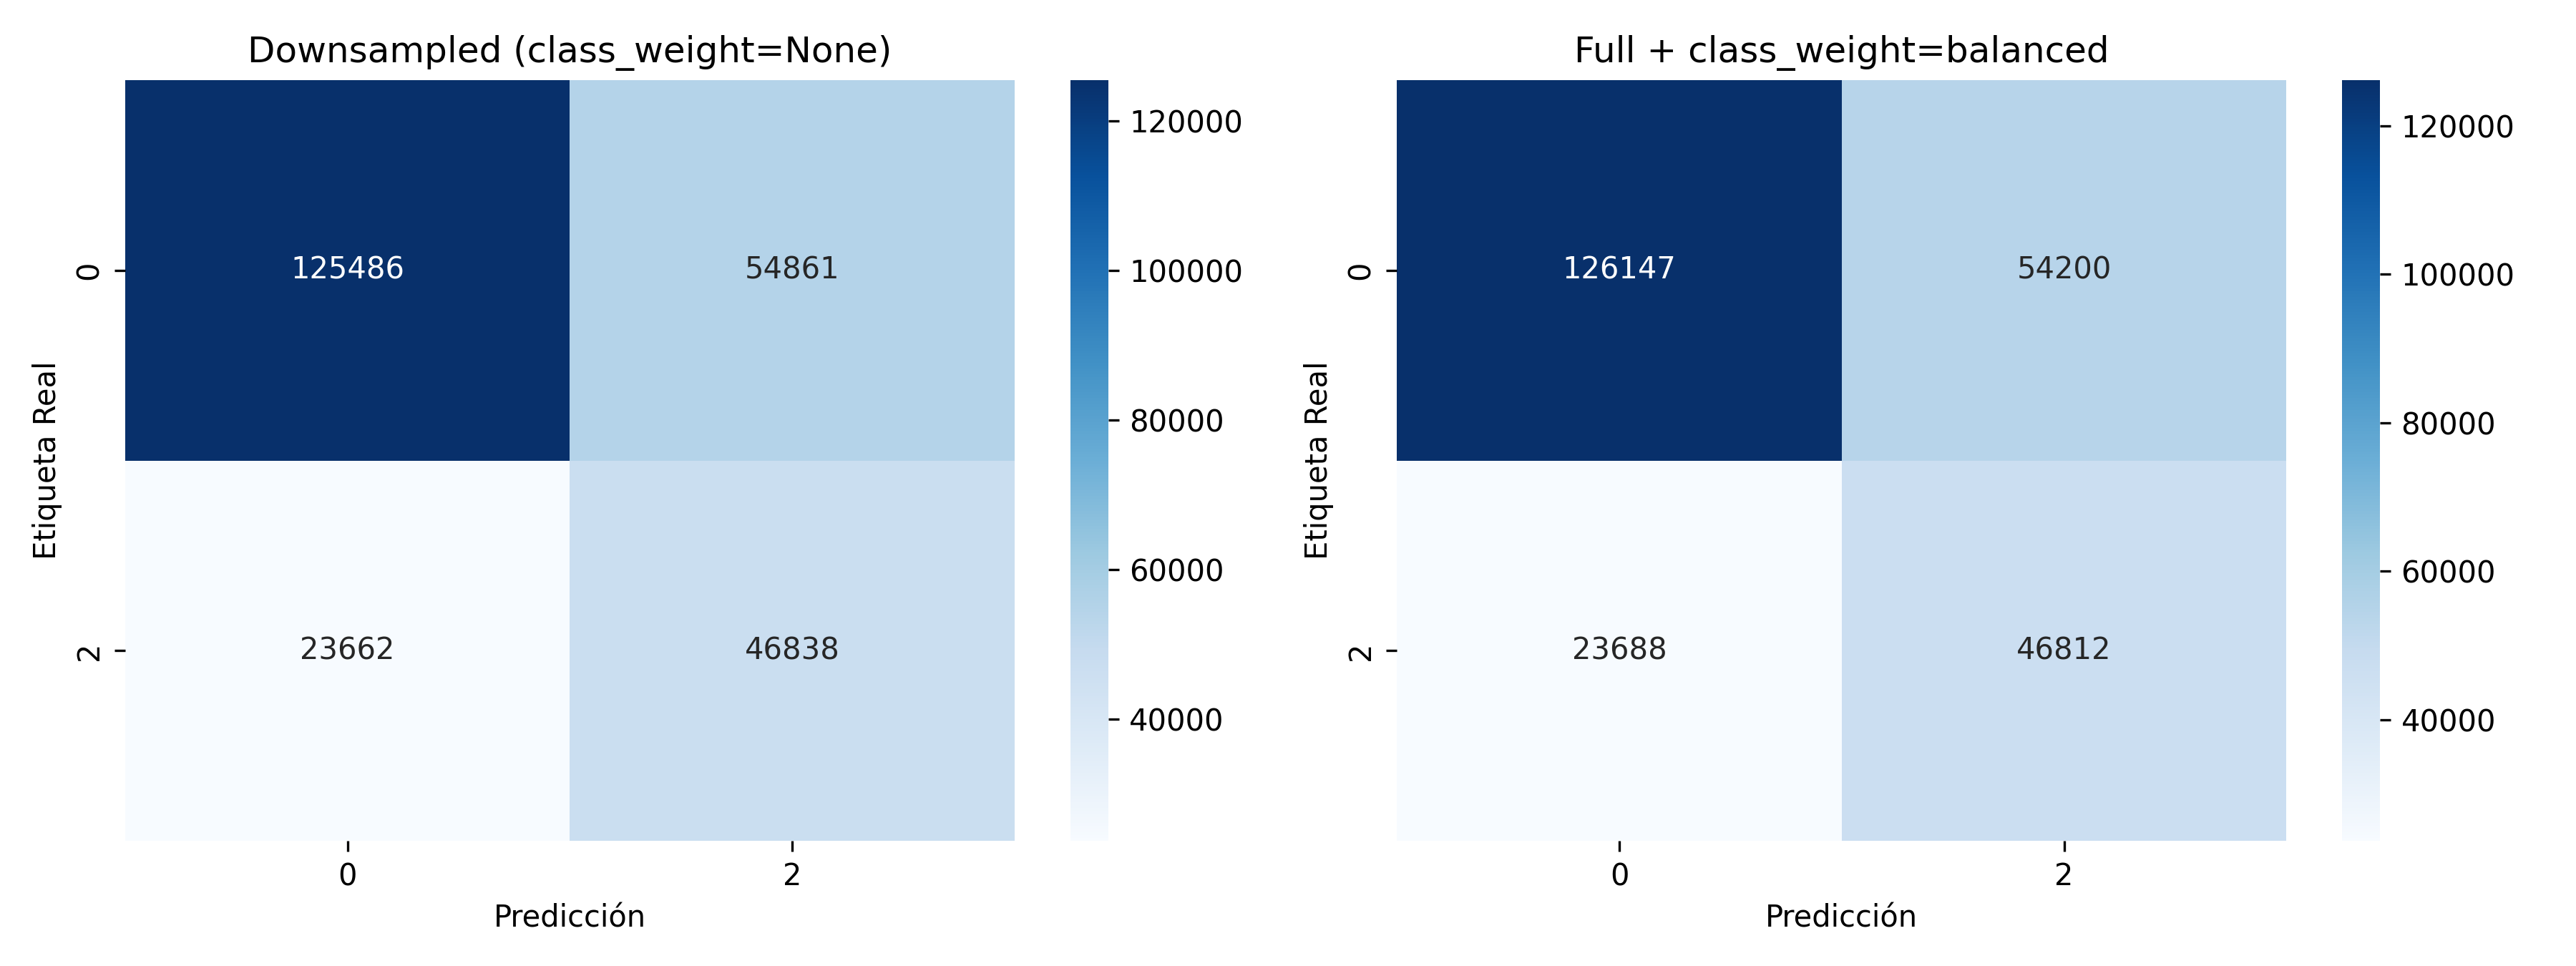
\includegraphics[width=0.9\textwidth]{baseline_downsampled_confusion_matrix.png}
    \caption{Matrices de confusión de las Regresiones Logísticas mono (submuestreo y ponderación).}
    \label{fig:cm_baseline}
\end{figure}

\subsection{Disponibilidad de código y datos}
El código se distribuye bajo licencia MIT en el repositorio \url{https://github.com/giulicrenna/Deteccion-Temprana-Depresion}. Los corpus de origen no se redistribuyen y deben descargarse desde sus fuentes, respetando sus licencias: Coello-Guilarte (uso de investigación con cita), Kaggle SDD (CC BY-SA 4.0), Reddit Mental Health Posts (sin licencia declarada) y Depression Reddit Cleaned (CC BY 4.0).

\end{document}
